% Options for packages loaded elsewhere
% Options for packages loaded elsewhere
\PassOptionsToPackage{unicode}{hyperref}
\PassOptionsToPackage{hyphens}{url}
\PassOptionsToPackage{dvipsnames,svgnames,x11names}{xcolor}
%
\documentclass[
  11pt,
  a4paper,
  onecolumn]{article}
\usepackage{xcolor}
\usepackage[top=1in,left=1in,right=1in,bottom=1in]{geometry}
\usepackage{amsmath,amssymb}
\setcounter{secnumdepth}{-\maxdimen} % remove section numbering
\usepackage{iftex}
\ifPDFTeX
  \usepackage[T1]{fontenc}
  \usepackage[utf8]{inputenc}
  \usepackage{textcomp} % provide euro and other symbols
\else % if luatex or xetex
  \usepackage{unicode-math} % this also loads fontspec
  \defaultfontfeatures{Scale=MatchLowercase}
  \defaultfontfeatures[\rmfamily]{Ligatures=TeX,Scale=1}
\fi
\usepackage{lmodern}
\ifPDFTeX\else
  % xetex/luatex font selection
\fi
% Use upquote if available, for straight quotes in verbatim environments
\IfFileExists{upquote.sty}{\usepackage{upquote}}{}
\IfFileExists{microtype.sty}{% use microtype if available
  \usepackage[]{microtype}
  \UseMicrotypeSet[protrusion]{basicmath} % disable protrusion for tt fonts
}{}
\usepackage{setspace}
\makeatletter
\@ifundefined{KOMAClassName}{% if non-KOMA class
  \IfFileExists{parskip.sty}{%
    \usepackage{parskip}
  }{% else
    \setlength{\parindent}{0pt}
    \setlength{\parskip}{6pt plus 2pt minus 1pt}}
}{% if KOMA class
  \KOMAoptions{parskip=half}}
\makeatother
% Make \paragraph and \subparagraph free-standing
\makeatletter
\ifx\paragraph\undefined\else
  \let\oldparagraph\paragraph
  \renewcommand{\paragraph}{
    \@ifstar
      \xxxParagraphStar
      \xxxParagraphNoStar
  }
  \newcommand{\xxxParagraphStar}[1]{\oldparagraph*{#1}\mbox{}}
  \newcommand{\xxxParagraphNoStar}[1]{\oldparagraph{#1}\mbox{}}
\fi
\ifx\subparagraph\undefined\else
  \let\oldsubparagraph\subparagraph
  \renewcommand{\subparagraph}{
    \@ifstar
      \xxxSubParagraphStar
      \xxxSubParagraphNoStar
  }
  \newcommand{\xxxSubParagraphStar}[1]{\oldsubparagraph*{#1}\mbox{}}
  \newcommand{\xxxSubParagraphNoStar}[1]{\oldsubparagraph{#1}\mbox{}}
\fi
\makeatother

\usepackage{color}
\usepackage{fancyvrb}
\newcommand{\VerbBar}{|}
\newcommand{\VERB}{\Verb[commandchars=\\\{\}]}
\DefineVerbatimEnvironment{Highlighting}{Verbatim}{commandchars=\\\{\}}
% Add ',fontsize=\small' for more characters per line
\newenvironment{Shaded}{}{}
\newcommand{\AlertTok}[1]{\textcolor[rgb]{1.00,0.33,0.33}{\textbf{#1}}}
\newcommand{\AnnotationTok}[1]{\textcolor[rgb]{0.42,0.45,0.49}{#1}}
\newcommand{\AttributeTok}[1]{\textcolor[rgb]{0.84,0.23,0.29}{#1}}
\newcommand{\BaseNTok}[1]{\textcolor[rgb]{0.00,0.36,0.77}{#1}}
\newcommand{\BuiltInTok}[1]{\textcolor[rgb]{0.84,0.23,0.29}{#1}}
\newcommand{\CharTok}[1]{\textcolor[rgb]{0.01,0.18,0.38}{#1}}
\newcommand{\CommentTok}[1]{\textcolor[rgb]{0.42,0.45,0.49}{#1}}
\newcommand{\CommentVarTok}[1]{\textcolor[rgb]{0.42,0.45,0.49}{#1}}
\newcommand{\ConstantTok}[1]{\textcolor[rgb]{0.00,0.36,0.77}{#1}}
\newcommand{\ControlFlowTok}[1]{\textcolor[rgb]{0.84,0.23,0.29}{#1}}
\newcommand{\DataTypeTok}[1]{\textcolor[rgb]{0.84,0.23,0.29}{#1}}
\newcommand{\DecValTok}[1]{\textcolor[rgb]{0.00,0.36,0.77}{#1}}
\newcommand{\DocumentationTok}[1]{\textcolor[rgb]{0.42,0.45,0.49}{#1}}
\newcommand{\ErrorTok}[1]{\textcolor[rgb]{1.00,0.33,0.33}{\underline{#1}}}
\newcommand{\ExtensionTok}[1]{\textcolor[rgb]{0.84,0.23,0.29}{\textbf{#1}}}
\newcommand{\FloatTok}[1]{\textcolor[rgb]{0.00,0.36,0.77}{#1}}
\newcommand{\FunctionTok}[1]{\textcolor[rgb]{0.44,0.26,0.76}{#1}}
\newcommand{\ImportTok}[1]{\textcolor[rgb]{0.01,0.18,0.38}{#1}}
\newcommand{\InformationTok}[1]{\textcolor[rgb]{0.42,0.45,0.49}{#1}}
\newcommand{\KeywordTok}[1]{\textcolor[rgb]{0.84,0.23,0.29}{#1}}
\newcommand{\NormalTok}[1]{\textcolor[rgb]{0.14,0.16,0.18}{#1}}
\newcommand{\OperatorTok}[1]{\textcolor[rgb]{0.14,0.16,0.18}{#1}}
\newcommand{\OtherTok}[1]{\textcolor[rgb]{0.44,0.26,0.76}{#1}}
\newcommand{\PreprocessorTok}[1]{\textcolor[rgb]{0.84,0.23,0.29}{#1}}
\newcommand{\RegionMarkerTok}[1]{\textcolor[rgb]{0.42,0.45,0.49}{#1}}
\newcommand{\SpecialCharTok}[1]{\textcolor[rgb]{0.00,0.36,0.77}{#1}}
\newcommand{\SpecialStringTok}[1]{\textcolor[rgb]{0.01,0.18,0.38}{#1}}
\newcommand{\StringTok}[1]{\textcolor[rgb]{0.01,0.18,0.38}{#1}}
\newcommand{\VariableTok}[1]{\textcolor[rgb]{0.89,0.38,0.04}{#1}}
\newcommand{\VerbatimStringTok}[1]{\textcolor[rgb]{0.01,0.18,0.38}{#1}}
\newcommand{\WarningTok}[1]{\textcolor[rgb]{1.00,0.33,0.33}{#1}}

\usepackage{longtable,booktabs,array}
\usepackage{calc} % for calculating minipage widths
% Correct order of tables after \paragraph or \subparagraph
\usepackage{etoolbox}
\makeatletter
\patchcmd\longtable{\par}{\if@noskipsec\mbox{}\fi\par}{}{}
\makeatother
% Allow footnotes in longtable head/foot
\IfFileExists{footnotehyper.sty}{\usepackage{footnotehyper}}{\usepackage{footnote}}
\makesavenoteenv{longtable}
\usepackage{graphicx}
\makeatletter
\newsavebox\pandoc@box
\newcommand*\pandocbounded[1]{% scales image to fit in text height/width
  \sbox\pandoc@box{#1}%
  \Gscale@div\@tempa{\textheight}{\dimexpr\ht\pandoc@box+\dp\pandoc@box\relax}%
  \Gscale@div\@tempb{\linewidth}{\wd\pandoc@box}%
  \ifdim\@tempb\p@<\@tempa\p@\let\@tempa\@tempb\fi% select the smaller of both
  \ifdim\@tempa\p@<\p@\scalebox{\@tempa}{\usebox\pandoc@box}%
  \else\usebox{\pandoc@box}%
  \fi%
}
% Set default figure placement to htbp
\def\fps@figure{htbp}
\makeatother





\setlength{\emergencystretch}{3em} % prevent overfull lines

\providecommand{\tightlist}{%
  \setlength{\itemsep}{0pt}\setlength{\parskip}{0pt}}



 


\makeatletter
\@ifpackageloaded{caption}{}{\usepackage{caption}}
\AtBeginDocument{%
\ifdefined\contentsname
  \renewcommand*\contentsname{Table of contents}
\else
  \newcommand\contentsname{Table of contents}
\fi
\ifdefined\listfigurename
  \renewcommand*\listfigurename{List of Figures}
\else
  \newcommand\listfigurename{List of Figures}
\fi
\ifdefined\listtablename
  \renewcommand*\listtablename{List of Tables}
\else
  \newcommand\listtablename{List of Tables}
\fi
\ifdefined\figurename
  \renewcommand*\figurename{Figure}
\else
  \newcommand\figurename{Figure}
\fi
\ifdefined\tablename
  \renewcommand*\tablename{Table}
\else
  \newcommand\tablename{Table}
\fi
}
\@ifpackageloaded{float}{}{\usepackage{float}}
\floatstyle{ruled}
\@ifundefined{c@chapter}{\newfloat{codelisting}{h}{lop}}{\newfloat{codelisting}{h}{lop}[chapter]}
\floatname{codelisting}{Listing}
\newcommand*\listoflistings{\listof{codelisting}{List of Listings}}
\makeatother
\makeatletter
\makeatother
\makeatletter
\@ifpackageloaded{caption}{}{\usepackage{caption}}
\@ifpackageloaded{subcaption}{}{\usepackage{subcaption}}
\makeatother
\usepackage{bookmark}
\IfFileExists{xurl.sty}{\usepackage{xurl}}{} % add URL line breaks if available
\urlstyle{same}
\hypersetup{
  pdftitle={Full Bayesian hierarchical model with latent dynamic structure for stress reactivity and five EMA PID-5 trait domains},
  pdfauthor={Corrado Caudek},
  colorlinks=true,
  linkcolor={blue},
  filecolor={Maroon},
  citecolor={Blue},
  urlcolor={Blue},
  pdfcreator={LaTeX via pandoc}}


\title{Full Bayesian hierarchical model with latent dynamic structure
for stress reactivity and five EMA PID-5 trait domains}
\author{Corrado Caudek}
\date{}
\begin{document}
\maketitle


\setstretch{1}
\subsection{Dati PID-5 e ESI-BF
(baseline)}\label{dati-pid-5-e-esi-bf-baseline}

Le misure ``basali'' corrispondenti ai 5 domini del PID-5 sono state
calcolate \textbf{escludendo} i 15 item che vengono usati nelle
notifiche EMA.

\begin{Shaded}
\begin{Highlighting}[]
\CommentTok{\# Importa i punteggi ESI{-}BF (fattore di rischio psicologico globale)}
\CommentTok{\# e tiene solo un record per soggetto}
\NormalTok{esi\_bf }\OtherTok{\textless{}{-}}\NormalTok{ rio}\SpecialCharTok{::}\FunctionTok{import}\NormalTok{(}
\NormalTok{  here}\SpecialCharTok{::}\FunctionTok{here}\NormalTok{(}
    \StringTok{"data"}\NormalTok{,}
    \StringTok{"processed"}\NormalTok{,}
    \StringTok{"esi\_bf.csv"}
\NormalTok{  )}
\NormalTok{) }\SpecialCharTok{|\textgreater{}}
\NormalTok{  dplyr}\SpecialCharTok{::}\FunctionTok{distinct}\NormalTok{(user\_id, }\AttributeTok{.keep\_all =} \ConstantTok{TRUE}\NormalTok{) }\SpecialCharTok{|\textgreater{}} \CommentTok{\# Keep only distinct user\_id}
\NormalTok{  dplyr}\SpecialCharTok{::}\FunctionTok{select}\NormalTok{(user\_id, esi\_bf) }\CommentTok{\# Select relevant columns}

\CommentTok{\# Importa i punteggi del PID{-}5, escludendo gli item usati nell’EMA}
\NormalTok{pid5 }\OtherTok{\textless{}{-}}\NormalTok{ rio}\SpecialCharTok{::}\FunctionTok{import}\NormalTok{(}
\NormalTok{  here}\SpecialCharTok{::}\FunctionTok{here}\NormalTok{(}
    \StringTok{"data"}\NormalTok{,}
    \StringTok{"processed"}\NormalTok{,}
    \StringTok{"pid5.csv"}
\NormalTok{  )}
\NormalTok{) }\SpecialCharTok{|\textgreater{}}
\NormalTok{  dplyr}\SpecialCharTok{::}\FunctionTok{distinct}\NormalTok{(user\_id, }\AttributeTok{.keep\_all =} \ConstantTok{TRUE}\NormalTok{) }\SpecialCharTok{|\textgreater{}}  \CommentTok{\# Keep only distinct user\_id}
\NormalTok{  dplyr}\SpecialCharTok{::}\FunctionTok{select}\NormalTok{(user\_id, }\FunctionTok{starts\_with}\NormalTok{(}\StringTok{"domain\_"}\NormalTok{)) }\CommentTok{\# Select domain variables}

\CommentTok{\# Merge dei dati basali in un unico dataframe}
\NormalTok{df }\OtherTok{\textless{}{-}} \FunctionTok{left\_join}\NormalTok{(esi\_bf, pid5, }\AttributeTok{by =} \StringTok{"user\_id"}\NormalTok{)}
\end{Highlighting}
\end{Shaded}

\subsection{Pulizia iniziale dei dati}\label{pulizia-iniziale-dei-dati}

\begin{Shaded}
\begin{Highlighting}[]
\CommentTok{\# Elimina soggetti con risposte non affidabili (careless responding)}
\NormalTok{user\_id\_with\_careless\_responding }\OtherTok{\textless{}{-}} \FunctionTok{c}\NormalTok{(}
  \StringTok{"ma\_se\_2005\_11\_14\_490"}\NormalTok{,}
  \StringTok{"reve20041021036"}\NormalTok{,}
  \StringTok{"di\_ma\_2005\_10\_20\_756"}\NormalTok{,}
  \StringTok{"pa\_sc\_2005\_09\_10\_468"}\NormalTok{,}
  \StringTok{"il\_re\_2006\_01\_18\_645"}\NormalTok{,}
  \StringTok{"so\_ma\_2003\_10\_13\_804"}\NormalTok{,}
  \StringTok{"lo\_ca\_2005\_05\_07\_05\_437"}\NormalTok{,}
  \StringTok{"va\_ma\_2005\_05\_31\_567"}\NormalTok{,}
  \StringTok{"no\_un\_2005\_06\_29\_880"}\NormalTok{,}
  \StringTok{"an\_bo\_1988\_08\_24\_166"}\NormalTok{,}
  \StringTok{"st\_ma\_2004\_04\_21\_426"}\NormalTok{,}
  \StringTok{"an\_st\_2005\_10\_16\_052"}\NormalTok{,}
  \StringTok{"vi\_de\_2002\_12\_30\_067"}\NormalTok{,}
  \StringTok{"gi\_ru\_2005\_03\_08\_033"}\NormalTok{,}
  \StringTok{"al\_mi\_2005\_03\_05\_844"}\NormalTok{,}
  \StringTok{"la\_ma\_2006\_01\_31\_787"}\NormalTok{,}
  \StringTok{"gi\_lo\_2004\_06\_27\_237"}\NormalTok{,}
  \StringTok{"ch\_bi\_2001\_01\_28\_407"}\NormalTok{,}
  \StringTok{"al\_pe\_2001\_04\_20\_079"}\NormalTok{,}
  \StringTok{"le\_de\_2003\_09\_05\_067"}\NormalTok{,}
  \StringTok{"fe\_gr\_2002\_02\_19\_434"}\NormalTok{,}
  \StringTok{"ma\_ba\_2002\_09\_09\_052"}\NormalTok{,}
  \StringTok{"ca\_gi\_2003\_09\_16\_737"}\NormalTok{,}
  \StringTok{"an\_to\_2003\_08\_06\_114"}\NormalTok{,}
  \StringTok{"al\_se\_2003\_07\_28\_277"}\NormalTok{,}
  \StringTok{"ja\_tr\_2002\_10\_06\_487"}\NormalTok{,}
  \StringTok{"el\_ci\_2002\_02\_15\_057"}\NormalTok{,}
  \StringTok{"se\_ti\_2000\_03\_04\_975"}\NormalTok{,}
  \StringTok{"co\_ga\_2003\_10\_29\_614"}\NormalTok{,}
  \StringTok{"al\_ba\_2003\_18\_07\_905"}\NormalTok{,}
  \StringTok{"bi\_ro\_2003\_09\_07\_934"}\NormalTok{,}
  \StringTok{"an\_va\_2004\_04\_08\_527"}\NormalTok{,}
  \StringTok{"ev\_cr\_2003\_01\_27\_573"}
\NormalTok{)}

\CommentTok{\# Filter out users with careless responses}
\NormalTok{df1 }\OtherTok{\textless{}{-}}\NormalTok{ df[}\SpecialCharTok{!}\NormalTok{(df}\SpecialCharTok{$}\NormalTok{user\_id }\SpecialCharTok{\%in\%}\NormalTok{ user\_id\_with\_careless\_responding), ]}
\end{Highlighting}
\end{Shaded}

\subsection{Caricamento dati EMA}\label{caricamento-dati-ema}

\begin{Shaded}
\begin{Highlighting}[]
\CommentTok{\# Legge i dati grezzi EMA e li unisce ai dati baseline}
\NormalTok{ema\_raw }\OtherTok{\textless{}{-}} \FunctionTok{readRDS}\NormalTok{(}
\NormalTok{  here}\SpecialCharTok{::}\FunctionTok{here}\NormalTok{(}
    \StringTok{"data"}\NormalTok{,}
    \StringTok{"raw"}\NormalTok{,}
    \StringTok{"ema"}\NormalTok{,}
    \StringTok{"ema\_data\_scoring.RDS"}
\NormalTok{  )}
\NormalTok{) }\SpecialCharTok{|\textgreater{}}
\NormalTok{  dplyr}\SpecialCharTok{::}\FunctionTok{rename}\NormalTok{(}
    \AttributeTok{user\_id =}\NormalTok{ subj\_code}
\NormalTok{  )}

\CommentTok{\# Merge EMA data with filtered main data}
\NormalTok{df2 }\OtherTok{\textless{}{-}} \FunctionTok{left\_join}\NormalTok{(df1, ema\_raw, }\AttributeTok{by =} \StringTok{"user\_id"}\NormalTok{)}

\CommentTok{\# Verify number of unique users}
\FunctionTok{length}\NormalTok{(}\FunctionTok{unique}\NormalTok{(df2}\SpecialCharTok{$}\NormalTok{user\_id))}
\end{Highlighting}
\end{Shaded}

\begin{verbatim}
[1] 429
\end{verbatim}

\begin{Shaded}
\begin{Highlighting}[]
\CommentTok{\# Conta quante risposte EMA ha fornito ciascun soggetto}
\NormalTok{user\_counts }\OtherTok{\textless{}{-}}\NormalTok{ df2 }\SpecialCharTok{\%\textgreater{}\%}
  \FunctionTok{group\_by}\NormalTok{(user\_id) }\SpecialCharTok{\%\textgreater{}\%}
  \FunctionTok{summarise}\NormalTok{(}\AttributeTok{n\_responses =} \FunctionTok{n}\NormalTok{()) }\SpecialCharTok{\%\textgreater{}\%}
  \FunctionTok{ungroup}\NormalTok{()}

\NormalTok{valid\_users }\OtherTok{\textless{}{-}}\NormalTok{ user\_counts }\SpecialCharTok{\%\textgreater{}\%}
  \FunctionTok{filter}\NormalTok{(n\_responses }\SpecialCharTok{\textgreater{}=} \DecValTok{10}\NormalTok{) }\SpecialCharTok{\%\textgreater{}\%}
  \FunctionTok{pull}\NormalTok{(user\_id)}

\CommentTok{\# Tiene solo i soggetti con almeno 10 risposte EMA}
\NormalTok{df2 }\OtherTok{\textless{}{-}}\NormalTok{ df2 }\SpecialCharTok{\%\textgreater{}\%}
\NormalTok{  dplyr}\SpecialCharTok{::}\FunctionTok{filter}\NormalTok{(user\_id }\SpecialCharTok{\%in\%}\NormalTok{ valid\_users)}
\end{Highlighting}
\end{Shaded}

\begin{Shaded}
\begin{Highlighting}[]
\FunctionTok{length}\NormalTok{(}\FunctionTok{unique}\NormalTok{(df2}\SpecialCharTok{$}\NormalTok{user\_id))}
\end{Highlighting}
\end{Shaded}

\begin{verbatim}
[1] 379
\end{verbatim}

\begin{Shaded}
\begin{Highlighting}[]
\FunctionTok{glimpse}\NormalTok{(df2)}
\end{Highlighting}
\end{Shaded}

\begin{verbatim}
Rows: 10,024
Columns: 89
$ user_id                   <chr> "an_ra_2004_06_07_770", "an_ra_2004_06_07_77~
$ esi_bf                    <int> 8, 8, 8, 8, 8, 8, 8, 8, 8, 8, 8, 8, 8, 8, 8,~
$ domain_negative_affect    <int> 35, 35, 35, 35, 35, 35, 35, 35, 35, 35, 35, ~
$ domain_detachment         <int> 18, 18, 18, 18, 18, 18, 18, 18, 18, 18, 18, ~
$ domain_antagonism         <int> 18, 18, 18, 18, 18, 18, 18, 18, 18, 18, 18, ~
$ domain_disinhibition      <int> 23, 23, 23, 23, 23, 23, 23, 23, 23, 23, 23, ~
$ domain_psychoticism       <int> 26, 26, 26, 26, 26, 26, 26, 26, 26, 26, 26, ~
$ happy                     <dbl> 61, 100, 77, 100, 35, 15, 29, 46, 74, 81, 22~
$ sad                       <dbl> 16, 0, 10, 10, 65, 62, 39, 52, 24, 10, 66, 7~
$ satisfied                 <dbl> 56, 100, 84, 91, 42, 20, 36, 19, 76, 88, 13,~
$ angry                     <dbl> 0, 0, 0, 0, 19, 26, 50, 67, 7, 14, 22, 50, 8~
$ pid5_13                   <dbl> 0, 1, 2, 1, 0, 0, 0, 0, 0, 0, 0, 2, 0, 0, 0,~
$ pid5_15                   <dbl> 2, 0, 0, 0, 0, 0, 0, 0, 0, 0, 0, 1, 0, 0, 0,~
$ pid5_11                   <dbl> 2, 2, 2, 0, 2, 2, 0, 0, 0, 0, 2, 2, 1, 0, 0,~
$ pid5_3                    <dbl> 1, 1, 3, 2, 2, 0, 0, 0, 0, 0, 2, 2, 2, 2, 0,~
$ pid5_2                    <dbl> 2, 2, 1, 0, 2, 2, 0, 3, 0, 0, 0, 1, 2, 0, 0,~
$ pid5_7                    <dbl> 2, 0, 1, 0, 0, 0, 0, 0, 0, 0, 0, 0, 0, 0, 0,~
$ pid5_14                   <dbl> 0, 1, 1, 0, 0, 0, 0, 0, 0, 0, 0, 0, 0, 0, 0,~
$ pid5_6                    <dbl> 2, 3, 2, 3, 3, 3, 3, 3, 3, 3, 3, 3, 3, 3, 2,~
$ pid5_4                    <dbl> 2, 3, 0, 0, 0, 1, 0, 0, 0, 0, 0, 0, 0, 0, 0,~
$ pid5_12                   <dbl> 1, 2, 1, 1, 0, 0, 0, 0, 0, 0, 1, 0, 0, 0, 0,~
$ pid5_1                    <dbl> 2, 2, 0, 0, 1, 1, 0, 2, 0, 0, 2, 2, 1, 0, 0,~
$ pid5_9                    <dbl> 1, 3, 0, 0, 0, 0, 0, 0, 0, 0, 0, 0, 0, 0, 0,~
$ pid5_5                    <dbl> 2, 2, 3, 0, 0, 0, 0, 0, 0, 0, 2, 1, 2, 2, 0,~
$ pid5_8                    <dbl> 0, 0, 0, 0, 0, 0, 0, 0, 0, 0, 0, 0, 0, 0, 0,~
$ pid5_10                   <dbl> 1, 3, 1, 1, 0, 0, 0, 0, 0, 0, 0, 1, 0, 0, 0,~
$ tripm_1                   <dbl> 2, 1, 4, 1, 2, 1, 1, 1, 1, 1, 1, 1, 1, 1, 1,~
$ tripm_3                   <dbl> 3, 1, 1, 1, 1, 1, 4, 1, 1, 1, 1, 1, 1, 1, 1,~
$ tripm_2                   <dbl> 1, 1, 1, 1, 1, 1, 1, 1, 1, 1, 1, 1, 1, 1, 1,~
$ tripm_4                   <dbl> 4, 2, 3, 3, 3, 3, 3, 3, 3, 4, 3, 3, 4, 3, 3,~
$ dass21_2                  <dbl> 0, NA, 2, NA, 0, NA, NA, 0, 0, NA, 2, NA, 0,~
$ dass21_5                  <dbl> 1, NA, 0, NA, 0, NA, NA, 0, 0, NA, 0, NA, 0,~
$ dass21_3                  <dbl> 1, NA, 0, NA, 0, NA, NA, 0, 0, NA, 0, NA, 0,~
$ dass21_4                  <dbl> 1, NA, 0, NA, 0, NA, NA, 2, 0, NA, 0, NA, 0,~
$ dass21_6                  <dbl> 0, NA, 0, NA, 0, NA, NA, 0, 0, NA, 0, NA, 0,~
$ dass21_1                  <dbl> 0, NA, 2, NA, 0, NA, NA, 1, 0, NA, 0, NA, 0,~
$ scs3_pos                  <dbl> 3, NA, 3, NA, 3, NA, NA, 3, -3, NA, -3, NA, ~
$ scs5_neg                  <dbl> -3, NA, -1, NA, -2, NA, NA, -2, -3, NA, -2, ~
$ scs7_pos                  <dbl> 1, NA, 2, NA, 2, NA, NA, 2, 1, NA, 2, NA, -1~
$ scs4_neg                  <dbl> 2, NA, 2, NA, -3, NA, NA, -3, -2, NA, 2, NA,~
$ scs2_neg                  <dbl> -1, NA, -2, NA, -3, NA, NA, -3, -3, NA, 2, N~
$ scs1_pos                  <dbl> -1, NA, 3, NA, 2, NA, NA, 2, -3, NA, 2, NA, ~
$ scs8_neg                  <dbl> 1, NA, 2, NA, -2, NA, NA, -3, -1, NA, 1, NA,~
$ scs6_pos                  <dbl> 1, NA, 2, NA, 2, NA, NA, 2, 2, NA, 2, NA, -3~
$ vq_2                      <dbl> NA, 0, NA, 0, NA, 0, 0, 0, 0, 0, NA, 0, NA, ~
$ vq_1                      <dbl> NA, 0, NA, 0, NA, 0, 0, 0, 0, 0, NA, 0, NA, ~
$ vq_4                      <dbl> NA, 0, NA, 0, NA, 0, 0, 0, 0, 0, NA, 0, NA, ~
$ vq_3                      <dbl> NA, 0, NA, 0, NA, 0, 0, 0, 0, 0, NA, 0, NA, ~
$ cope_nvi_2                <dbl> NA, 4, NA, 2, NA, 2, 1, 3, 1, 2, NA, 1, NA, ~
$ cope_nvi_7                <dbl> NA, 4, NA, 2, NA, 3, 4, 4, 3, 4, NA, 2, NA, ~
$ cope_nvi_5                <dbl> NA, 4, NA, 3, NA, 4, 3, 4, 3, 4, NA, 4, NA, ~
$ cope_nvi_8                <dbl> NA, 4, NA, 3, NA, 4, 3, 4, 4, 4, NA, 3, NA, ~
$ cope_nvi_9                <dbl> NA, 1, NA, 1, NA, 1, 1, 1, 1, 1, NA, 1, NA, ~
$ cope_nvi_10               <dbl> NA, 1, NA, 1, NA, 1, 2, 1, 1, 1, NA, 4, NA, ~
$ cope_nvi_1                <dbl> NA, 2, NA, 1, NA, 1, 1, 1, 1, 1, NA, 1, NA, ~
$ cope_nvi_3                <dbl> NA, 3, NA, 3, NA, 3, 3, 4, 4, 4, NA, 2, NA, ~
$ cope_nvi_4                <dbl> NA, 4, NA, 3, NA, 3, 3, 4, 4, 4, NA, 2, NA, ~
$ cope_nvi_6                <dbl> NA, 4, NA, 3, NA, 4, 3, 4, 4, 4, NA, 4, NA, ~
$ day                       <date> 2025-03-22, 2025-03-26, 2025-03-29, 2025-04~
$ hour                      <int> 9, 18, 9, 18, 9, 18, 9, 21, 17, 18, 18, 11, ~
$ calendar_day              <dbl> 1, 2, 3, 4, 5, 6, 7, 8, 9, 10, 11, 12, 13, 1~
$ bysubj_day                <int> 1, 2, 3, 4, 5, 6, 7, 8, 9, 10, 11, 12, 13, 1~
$ context_quality           <dbl> 1, 2, 0, 2, 0, 0, -1, -1, 2, 2, -1, 0, -1, 1~
$ context_control           <dbl> 2, 4, 3, 5, 3, 2, 2, 2, 4, 5, 2, 2, 1, 4, 5,~
$ context_support           <dbl> 2, 2, 4, 3, 3, 2, 2, 5, 3, 5, 3, 3, 1, 3, 5,~
$ context_threat            <dbl> 1, 0, 1, 0, 1, 2, 1, 2, 0, 0, 2, 2, 2, 0, 1,~
$ pid5_sum                  <dbl> 20, 25, 17, 8, 10, 9, 3, 8, 3, 3, 12, 15, 11~
$ pid5_negative_affectivity <dbl> 5, 5, 4, 2, 5, 3, 0, 5, 0, 0, 4, 5, 5, 2, 0,~
$ pid5_detachment           <dbl> 6, 8, 5, 3, 3, 4, 3, 3, 3, 3, 5, 4, 5, 5, 2,~
$ pid5_antagonism           <dbl> 3, 3, 1, 0, 0, 0, 0, 0, 0, 0, 0, 0, 0, 0, 0,~
$ pid5_disinhibition        <dbl> 4, 7, 4, 2, 2, 2, 0, 0, 0, 0, 3, 3, 1, 0, 0,~
$ pid5_psychoticism         <dbl> 2, 2, 3, 1, 0, 0, 0, 0, 0, 0, 0, 3, 0, 0, 0,~
$ ipv_sum                   <dbl> NA, 0, NA, 0, NA, 0, 0, 0, 0, 0, NA, 0, NA, ~
$ tripm_4_rev               <dbl> 1, 3, 2, 2, 2, 2, 2, 2, 2, 1, 2, 2, 1, 2, 2,~
$ tripm_sum                 <dbl> 10, 5, 9, 6, 7, 6, 9, 6, 6, 7, 6, 6, 7, 6, 6~
$ tripm_boldness            <dbl> 3, 2, 5, 2, 3, 2, 2, 2, 2, 2, 2, 2, 2, 2, 2,~
$ tripm_meanness            <dbl> 4, 4, 3, 3, 3, 3, 6, 3, 3, 2, 3, 3, 2, 3, 3,~
$ dass_sum                  <dbl> 3, NA, 4, NA, 0, NA, NA, 3, 0, NA, 2, NA, 0,~
$ dass_stress               <dbl> 0, NA, 4, NA, 0, NA, NA, 1, 0, NA, 2, NA, 0,~
$ dass_depression           <dbl> 2, NA, 0, NA, 0, NA, NA, 2, 0, NA, 0, NA, 0,~
$ dass_anxiety              <dbl> 1, NA, 0, NA, 0, NA, NA, 0, 0, NA, 0, NA, 0,~
$ cope_10_rev               <dbl> NA, 4, NA, 4, NA, 4, 3, 4, 4, 4, NA, 1, NA, ~
$ cope_avoid                <dbl> NA, 6, NA, 3, NA, 3, 2, 4, 2, 3, NA, 2, NA, ~
$ cope_prob_or              <dbl> NA, 7, NA, 6, NA, 6, 6, 8, 8, 8, NA, 4, NA, ~
$ cope_social_support       <dbl> NA, 8, NA, 6, NA, 8, 6, 8, 7, 8, NA, 8, NA, ~
$ cope_positive_att         <dbl> NA, 8, NA, 5, NA, 7, 7, 8, 7, 8, NA, 5, NA, ~
$ cope_trascendent_or       <dbl> NA, 5, NA, 5, NA, 5, 4, 5, 5, 5, NA, 2, NA, ~
$ cs_pos                    <dbl> 4, NA, 10, NA, 9, NA, NA, 9, -3, NA, 3, NA, ~
$ ucs_neg                   <dbl> -1, NA, 1, NA, -10, NA, NA, -11, -9, NA, 3, ~
\end{verbatim}

\subsection{Costruzione della variabile
`exam\_period'}\label{costruzione-della-variabile-exam_period}

\begin{Shaded}
\begin{Highlighting}[]
\CommentTok{\# Importa i dati delle date d\textquotesingle{}esame per ogni soggetto}
\NormalTok{exam\_data }\OtherTok{\textless{}{-}}\NormalTok{ rio}\SpecialCharTok{::}\FunctionTok{import}\NormalTok{(}
\NormalTok{  here}\SpecialCharTok{::}\FunctionTok{here}\NormalTok{(}
    \StringTok{"data"}\NormalTok{, }\StringTok{"raw"}\NormalTok{, }\StringTok{"exam\_data.xlsx"}
\NormalTok{  )}
\NormalTok{) }\SpecialCharTok{\%\textgreater{}\%}
\NormalTok{  dplyr}\SpecialCharTok{::}\FunctionTok{select}\NormalTok{(}\AttributeTok{user\_id =}\NormalTok{ subj\_code, }\AttributeTok{exam\_day =}\NormalTok{ date, course, sex)}
\end{Highlighting}
\end{Shaded}

\begin{Shaded}
\begin{Highlighting}[]
\CommentTok{\# Pulisce le date e ne estrae la componente valida}
\NormalTok{exam\_data\_clean }\OtherTok{\textless{}{-}}\NormalTok{ exam\_data }\SpecialCharTok{\%\textgreater{}\%}
  \FunctionTok{mutate}\NormalTok{(}
    \CommentTok{\# Estrae solo la parte che somiglia a una data}
    \AttributeTok{exam\_day\_extracted =} \FunctionTok{str\_extract}\NormalTok{(exam\_day, }\StringTok{"}\SpecialCharTok{\textbackslash{}\textbackslash{}}\StringTok{b}\SpecialCharTok{\textbackslash{}\textbackslash{}}\StringTok{d\{1,2\}[{-}\_}\SpecialCharTok{\textbackslash{}\textbackslash{}}\StringTok{./]}\SpecialCharTok{\textbackslash{}\textbackslash{}}\StringTok{d\{1,2\}[{-}\_}\SpecialCharTok{\textbackslash{}\textbackslash{}}\StringTok{./]}\SpecialCharTok{\textbackslash{}\textbackslash{}}\StringTok{d\{2,4\}}\SpecialCharTok{\textbackslash{}\textbackslash{}}\StringTok{b"}\NormalTok{),}
    \CommentTok{\# Sostituisce separatori misti con "/"}
    \AttributeTok{exam\_day\_clean =} \FunctionTok{str\_replace\_all}\NormalTok{(exam\_day\_extracted, }\StringTok{"[{-}\_}\SpecialCharTok{\textbackslash{}\textbackslash{}}\StringTok{.]"}\NormalTok{, }\StringTok{"/"}\NormalTok{),}
    \CommentTok{\# Converte in formato Date}
    \AttributeTok{exam\_day\_date =} \FunctionTok{suppressWarnings}\NormalTok{(}\FunctionTok{dmy}\NormalTok{(exam\_day\_clean))}
\NormalTok{  )}
\end{Highlighting}
\end{Shaded}

\begin{Shaded}
\begin{Highlighting}[]
\CommentTok{\# Sostituisce le date per il corso Psicometria con quelle ufficiali}
\NormalTok{psicom\_dates }\OtherTok{\textless{}{-}} \FunctionTok{tibble}\NormalTok{(}
  \AttributeTok{exam\_day\_date =} \FunctionTok{as.Date}\NormalTok{(}\FunctionTok{c}\NormalTok{(}\StringTok{"2025{-}04{-}15"}\NormalTok{, }\StringTok{"2025{-}05{-}22"}\NormalTok{, }\StringTok{"2025{-}05{-}26"}\NormalTok{))}
\NormalTok{)}
\end{Highlighting}
\end{Shaded}

\begin{Shaded}
\begin{Highlighting}[]
\NormalTok{exam\_data\_psicom }\OtherTok{\textless{}{-}}\NormalTok{ exam\_data\_clean }\SpecialCharTok{\%\textgreater{}\%}
\NormalTok{  dplyr}\SpecialCharTok{::}\FunctionTok{filter}\NormalTok{(course }\SpecialCharTok{==} \StringTok{"Psicometria"}\NormalTok{) }\SpecialCharTok{\%\textgreater{}\%}
\NormalTok{  dplyr}\SpecialCharTok{::}\FunctionTok{distinct}\NormalTok{(user\_id, course, sex) }\SpecialCharTok{\%\textgreater{}\%}
\NormalTok{  tidyr}\SpecialCharTok{::}\FunctionTok{crossing}\NormalTok{(psicom\_dates)}
\end{Highlighting}
\end{Shaded}

\begin{Shaded}
\begin{Highlighting}[]
\CommentTok{\# Mantiene dati validi per altri corsi (solo se la data è valida)}
\NormalTok{exam\_data\_other }\OtherTok{\textless{}{-}}\NormalTok{ exam\_data\_clean }\SpecialCharTok{\%\textgreater{}\%}
\NormalTok{  dplyr}\SpecialCharTok{::}\FunctionTok{filter}\NormalTok{(course }\SpecialCharTok{!=} \StringTok{"Psicometria"}\NormalTok{, }\SpecialCharTok{!}\FunctionTok{is.na}\NormalTok{(exam\_day\_date)) }\SpecialCharTok{\%\textgreater{}\%}
\NormalTok{  dplyr}\SpecialCharTok{::}\FunctionTok{select}\NormalTok{(user\_id, course, sex, exam\_day\_date)}
\end{Highlighting}
\end{Shaded}

\begin{Shaded}
\begin{Highlighting}[]
\CommentTok{\# Unisce i due}
\NormalTok{exam\_data\_fixed }\OtherTok{\textless{}{-}} \FunctionTok{bind\_rows}\NormalTok{(exam\_data\_psicom, exam\_data\_other)}
\end{Highlighting}
\end{Shaded}

\begin{Shaded}
\begin{Highlighting}[]
\CommentTok{\# Estrae le date, corregge il formato, e crea variabili per: giorno prima, }
\CommentTok{\# giorno dopo, giorno esame}
\NormalTok{exam\_data\_long }\OtherTok{\textless{}{-}}\NormalTok{ exam\_data\_fixed }\SpecialCharTok{\%\textgreater{}\%}
  \FunctionTok{mutate}\NormalTok{(}
    \AttributeTok{pre\_exam\_1 =}\NormalTok{ exam\_day\_date }\SpecialCharTok{{-}} \FunctionTok{days}\NormalTok{(}\DecValTok{1}\NormalTok{),}
    \AttributeTok{pre\_exam\_2 =}\NormalTok{ exam\_day\_date }\SpecialCharTok{{-}} \FunctionTok{days}\NormalTok{(}\DecValTok{2}\NormalTok{),}
    \AttributeTok{post\_exam =}\NormalTok{ exam\_day\_date }\SpecialCharTok{+} \FunctionTok{days}\NormalTok{(}\DecValTok{1}\NormalTok{)}
\NormalTok{  ) }\SpecialCharTok{\%\textgreater{}\%}
\NormalTok{  dplyr}\SpecialCharTok{::}\FunctionTok{select}\NormalTok{(user\_id, pre\_exam\_1, pre\_exam\_2, }\AttributeTok{exam\_day =}\NormalTok{ exam\_day\_date, post\_exam) }\SpecialCharTok{\%\textgreater{}\%}
  \FunctionTok{pivot\_longer}\NormalTok{(}
    \AttributeTok{cols =} \FunctionTok{c}\NormalTok{(pre\_exam\_1, pre\_exam\_2, exam\_day, post\_exam),}
    \AttributeTok{names\_to =} \StringTok{"exam\_period\_raw"}\NormalTok{,}
    \AttributeTok{values\_to =} \StringTok{"exam\_date"}
\NormalTok{  ) }\SpecialCharTok{\%\textgreater{}\%}
  \FunctionTok{mutate}\NormalTok{(}
    \AttributeTok{exam\_period =} \FunctionTok{case\_when}\NormalTok{(}
\NormalTok{      exam\_period\_raw }\SpecialCharTok{\%in\%} \FunctionTok{c}\NormalTok{(}\StringTok{"pre\_exam\_1"}\NormalTok{, }\StringTok{"pre\_exam\_2"}\NormalTok{) }\SpecialCharTok{\textasciitilde{}} \StringTok{"pre\_exam"}\NormalTok{,}
\NormalTok{      exam\_period\_raw }\SpecialCharTok{\%in\%} \FunctionTok{c}\NormalTok{(}\StringTok{"exam\_day"}\NormalTok{, }\StringTok{"post\_exam"}\NormalTok{) }\SpecialCharTok{\textasciitilde{}} \StringTok{"post\_exam"}
\NormalTok{    )}
\NormalTok{  )}
\end{Highlighting}
\end{Shaded}

\begin{Shaded}
\begin{Highlighting}[]
\CommentTok{\# Unisce le informazioni EMA e d\textquotesingle{}esame in un unico dataframe}
\NormalTok{df\_exam\_tagged }\OtherTok{\textless{}{-}}\NormalTok{ df2 }\SpecialCharTok{\%\textgreater{}\%}
  \FunctionTok{left\_join}\NormalTok{(exam\_data\_long, }
            \AttributeTok{by =} \FunctionTok{c}\NormalTok{(}\StringTok{"user\_id"} \OtherTok{=} \StringTok{"user\_id"}\NormalTok{, }\StringTok{"day"} \OtherTok{=} \StringTok{"exam\_date"}\NormalTok{)) }\SpecialCharTok{\%\textgreater{}\%}
  \FunctionTok{mutate}\NormalTok{(}
    \AttributeTok{exam\_period =} \FunctionTok{coalesce}\NormalTok{(exam\_period, }\StringTok{"baseline"}\NormalTok{)  }\CommentTok{\# se NA, è "baseline"}
\NormalTok{  )}
\end{Highlighting}
\end{Shaded}

\begin{Shaded}
\begin{Highlighting}[]
\FunctionTok{table}\NormalTok{(df\_exam\_tagged}\SpecialCharTok{$}\NormalTok{exam\_period)}
\end{Highlighting}
\end{Shaded}

\begin{verbatim}

 baseline post_exam  pre_exam 
     8879       602       543 
\end{verbatim}

\subsection{\texorpdfstring{Variabile binaria
\texttt{under\_stress}}{Variabile binaria under\_stress}}\label{variabile-binaria-under_stress}

\begin{Shaded}
\begin{Highlighting}[]
\NormalTok{df\_exam\_tagged }\OtherTok{\textless{}{-}}\NormalTok{ df\_exam\_tagged }\SpecialCharTok{\%\textgreater{}\%}
  \FunctionTok{mutate}\NormalTok{(}\AttributeTok{under\_stress =} \FunctionTok{if\_else}\NormalTok{(exam\_period }\SpecialCharTok{\%in\%} \FunctionTok{c}\NormalTok{(}\StringTok{"pre\_exam"}\NormalTok{, }\StringTok{"post\_exam"}\NormalTok{), }\DecValTok{1}\NormalTok{, }\DecValTok{0}\NormalTok{))}
\end{Highlighting}
\end{Shaded}

In questo script la variabile \texttt{under\_stress} non viene usata.

\subsection{Calcolo affetto negativo
istantaneo}\label{calcolo-affetto-negativo-istantaneo}

\begin{Shaded}
\begin{Highlighting}[]
\CommentTok{\# Costruisce una misura media dell\textquotesingle{}affetto negativo momentaneo}

\CommentTok{\# Seleziona solo le colonne rilevanti (per velocità)}
\NormalTok{items }\OtherTok{\textless{}{-}} \FunctionTok{c}\NormalTok{(}\StringTok{"sad"}\NormalTok{, }\StringTok{"angry"}\NormalTok{, }\StringTok{"happy"}\NormalTok{, }\StringTok{"satisfied"}\NormalTok{)}

\CommentTok{\# Imputazione dei missing su variabili di umore}
\NormalTok{imputed }\OtherTok{\textless{}{-}} \FunctionTok{mice}\NormalTok{(df\_exam\_tagged[, items], }\AttributeTok{m =} \DecValTok{1}\NormalTok{, }\AttributeTok{maxit =} \DecValTok{10}\NormalTok{, }\AttributeTok{seed =} \DecValTok{123}\NormalTok{)}
\end{Highlighting}
\end{Shaded}

\begin{verbatim}

 iter imp variable
  1   1  sad  angry  happy  satisfied
  2   1  sad  angry  happy  satisfied
  3   1  sad  angry  happy  satisfied
  4   1  sad  angry  happy  satisfied
  5   1  sad  angry  happy  satisfied
  6   1  sad  angry  happy  satisfied
  7   1  sad  angry  happy  satisfied
  8   1  sad  angry  happy  satisfied
  9   1  sad  angry  happy  satisfied
  10   1  sad  angry  happy  satisfied
\end{verbatim}

\begin{Shaded}
\begin{Highlighting}[]
\CommentTok{\# Estrai il dataset imputato e sostituisci le colonne originali}
\NormalTok{df2\_imputed }\OtherTok{\textless{}{-}} \FunctionTok{complete}\NormalTok{(imputed)}
\NormalTok{df2[, items] }\OtherTok{\textless{}{-}}\NormalTok{ df2\_imputed[, items]}

\CommentTok{\# Calcolo della media invertendo happy/satisfied}
\NormalTok{df\_exam\_tagged }\OtherTok{\textless{}{-}}\NormalTok{ df\_exam\_tagged }\SpecialCharTok{\%\textgreater{}\%}
  \FunctionTok{mutate}\NormalTok{(}
    \AttributeTok{happy\_reversed =} \DecValTok{100} \SpecialCharTok{{-}}\NormalTok{ happy, }\CommentTok{\# Scala 0{-}100}
    \AttributeTok{satisfied\_reversed =} \DecValTok{100} \SpecialCharTok{{-}}\NormalTok{ satisfied,}
    \AttributeTok{neg\_aff\_ema =} \FunctionTok{rowMeans}\NormalTok{(}
      \FunctionTok{cbind}\NormalTok{(sad, angry, happy\_reversed, satisfied\_reversed),}
      \AttributeTok{na.rm =} \ConstantTok{TRUE}
\NormalTok{    )}
\NormalTok{  )}
\end{Highlighting}
\end{Shaded}

\subsection{\texorpdfstring{Variabili \texttt{delta\_ucs} e
\texttt{delta\_mood}}{Variabili delta\_ucs e delta\_mood}}\label{variabili-delta_ucs-e-delta_mood}

Se i valori di pre-esame sono più alti della baseline e i valori di
post-esame sono più bassi della baseline, allora la formula (post - pre)
/ baseline potrebbe effettivamente catturare meglio l'effetto
complessivo dello stress.

\begin{itemize}
\tightlist
\item
  (post - pre) cattura la direzione del cambiamento (se i valori stanno
  diminuendo o aumentando);
\item
  La divisione per baseline normalizza il cambiamento rispetto al
  livello basale, rendendo l'effetto comparabile tra soggetti con
  diversi livelli di partenza.
\end{itemize}

\begin{Shaded}
\begin{Highlighting}[]
\CommentTok{\# df\_stress\_effects \textless{}{-} df\_exam\_tagged \%\textgreater{}\%}
\CommentTok{\#   dplyr::filter(exam\_period \%in\% c("baseline", "post\_exam")) \%\textgreater{}\%}
\CommentTok{\#   group\_by(user\_id, exam\_period) \%\textgreater{}\%}
\CommentTok{\#   summarise(}
\CommentTok{\#     ucs = mean(ucs\_neg, na.rm = TRUE),}
\CommentTok{\#     mood = mean(neg\_aff\_ema, na.rm = TRUE),}
\CommentTok{\#     .groups = "drop"}
\CommentTok{\#   ) \%\textgreater{}\%}
\CommentTok{\#   pivot\_wider(names\_from = exam\_period, values\_from = c(ucs, mood)) \%\textgreater{}\%}
\CommentTok{\#   mutate(}
\CommentTok{\#     delta\_ucs = ucs\_post\_exam {-} ucs\_baseline,}
\CommentTok{\#     delta\_mood = mood\_post\_exam {-} mood\_baseline}
\CommentTok{\#   )}

\NormalTok{df\_stress\_effects }\OtherTok{\textless{}{-}}\NormalTok{ df\_exam\_tagged }\SpecialCharTok{\%\textgreater{}\%}
\NormalTok{  dplyr}\SpecialCharTok{::}\FunctionTok{filter}\NormalTok{(exam\_period }\SpecialCharTok{\%in\%} \FunctionTok{c}\NormalTok{(}\StringTok{"baseline"}\NormalTok{, }\StringTok{"pre\_exam"}\NormalTok{, }\StringTok{"post\_exam"}\NormalTok{)) }\SpecialCharTok{\%\textgreater{}\%}
  \FunctionTok{group\_by}\NormalTok{(user\_id, exam\_period) }\SpecialCharTok{\%\textgreater{}\%}
  \FunctionTok{summarise}\NormalTok{(}
    \AttributeTok{ucs =} \FunctionTok{mean}\NormalTok{(ucs\_neg, }\AttributeTok{na.rm =} \ConstantTok{TRUE}\NormalTok{),}
    \AttributeTok{mood =} \FunctionTok{mean}\NormalTok{(neg\_aff\_ema, }\AttributeTok{na.rm =} \ConstantTok{TRUE}\NormalTok{),}
    \AttributeTok{.groups =} \StringTok{"drop"}
\NormalTok{  ) }\SpecialCharTok{\%\textgreater{}\%}
  \FunctionTok{pivot\_wider}\NormalTok{(}\AttributeTok{names\_from =}\NormalTok{ exam\_period, }\AttributeTok{values\_from =} \FunctionTok{c}\NormalTok{(ucs, mood)) }\SpecialCharTok{\%\textgreater{}\%}
  \FunctionTok{mutate}\NormalTok{(}
    \AttributeTok{delta\_ucs =}\NormalTok{ (ucs\_post\_exam }\SpecialCharTok{{-}}\NormalTok{ ucs\_pre\_exam) }\SpecialCharTok{/}\NormalTok{ ucs\_baseline,}
    \AttributeTok{delta\_mood =}\NormalTok{ (mood\_post\_exam }\SpecialCharTok{{-}}\NormalTok{ mood\_pre\_exam) }\SpecialCharTok{/}\NormalTok{ mood\_baseline}
\NormalTok{  )}
\end{Highlighting}
\end{Shaded}

Qui soltanto descrivo il pattern di cambiamento (pre/post) rispetto alla
baseline.

\begin{Shaded}
\begin{Highlighting}[]
\NormalTok{mod1 }\OtherTok{\textless{}{-}} \FunctionTok{brm}\NormalTok{(}
\NormalTok{  ucs\_neg }\SpecialCharTok{\textasciitilde{}}\NormalTok{ exam\_period }\SpecialCharTok{+}\NormalTok{ (}\DecValTok{1} \SpecialCharTok{+}\NormalTok{ exam\_period }\SpecialCharTok{|}\NormalTok{ user\_id),}
  \AttributeTok{data =}\NormalTok{ df\_exam\_tagged,}
  \AttributeTok{family =} \FunctionTok{gaussian}\NormalTok{(),}
  \AttributeTok{backend =} \StringTok{"cmdstanr"}
\NormalTok{)}
\end{Highlighting}
\end{Shaded}

\begin{Shaded}
\begin{Highlighting}[]
\FunctionTok{pp\_check}\NormalTok{(mod1)}
\end{Highlighting}
\end{Shaded}

\begin{verbatim}
Using 10 posterior draws for ppc type 'dens_overlay' by default.
\end{verbatim}

\pandocbounded{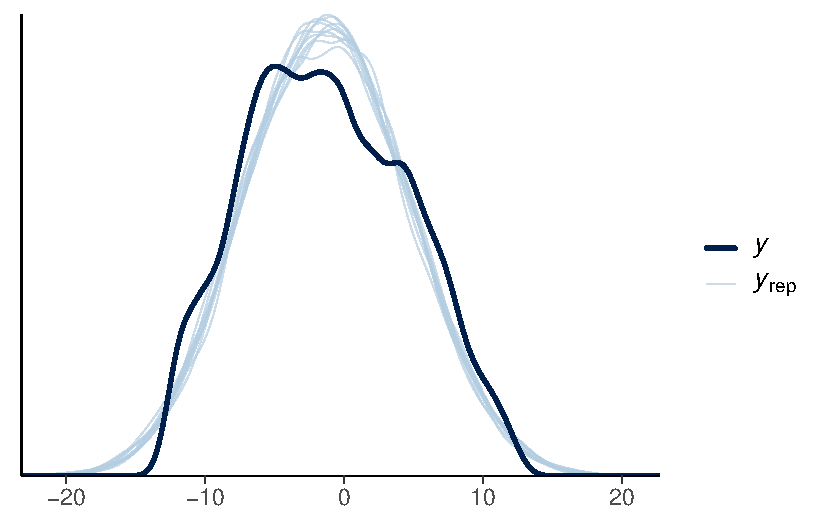
\includegraphics[keepaspectratio]{risk_files/figure-pdf/unnamed-chunk-20-1.pdf}}

\begin{Shaded}
\begin{Highlighting}[]
\FunctionTok{print}\NormalTok{(mod1)}
\end{Highlighting}
\end{Shaded}

\begin{verbatim}
 Family: gaussian 
  Links: mu = identity; sigma = identity 
Formula: ucs_neg ~ exam_period + (1 + exam_period | user_id) 
   Data: df_exam_tagged (Number of observations: 6229) 
  Draws: 4 chains, each with iter = 2000; warmup = 1000; thin = 1;
         total post-warmup draws = 4000

Multilevel Hyperparameters:
~user_id (Number of levels: 379) 
                                              Estimate Est.Error l-95% CI
sd(Intercept)                                     4.32      0.17     3.99
sd(exam_periodpost_exam)                          0.77      0.45     0.04
sd(exam_periodpre_exam)                           0.76      0.45     0.04
cor(Intercept,exam_periodpost_exam)              -0.16      0.30    -0.74
cor(Intercept,exam_periodpre_exam)                0.17      0.31    -0.49
cor(exam_periodpost_exam,exam_periodpre_exam)     0.29      0.48    -0.77
                                              u-95% CI Rhat Bulk_ESS Tail_ESS
sd(Intercept)                                     4.67 1.01      356     1090
sd(exam_periodpost_exam)                          1.65 1.01      403     1241
sd(exam_periodpre_exam)                           1.67 1.02      460     1389
cor(Intercept,exam_periodpost_exam)               0.53 1.00     3631     1586
cor(Intercept,exam_periodpre_exam)                0.80 1.01     3575     2061
cor(exam_periodpost_exam,exam_periodpre_exam)     0.94 1.00      660     1940

Regression Coefficients:
                     Estimate Est.Error l-95% CI u-95% CI Rhat Bulk_ESS
Intercept               -1.23      0.23    -1.67    -0.79 1.02      255
exam_periodpost_exam    -0.79      0.20    -1.18    -0.39 1.00     5065
exam_periodpre_exam      0.76      0.23     0.33     1.21 1.00     5578
                     Tail_ESS
Intercept                 440
exam_periodpost_exam     3080
exam_periodpre_exam      3249

Further Distributional Parameters:
      Estimate Est.Error l-95% CI u-95% CI Rhat Bulk_ESS Tail_ESS
sigma     3.88      0.04     3.81     3.95 1.00     4607     2880

Draws were sampled using sample(hmc). For each parameter, Bulk_ESS
and Tail_ESS are effective sample size measures, and Rhat is the potential
scale reduction factor on split chains (at convergence, Rhat = 1).
\end{verbatim}

\begin{Shaded}
\begin{Highlighting}[]
\FunctionTok{conditional\_effects}\NormalTok{(mod1, }\StringTok{"exam\_period"}\NormalTok{)}
\end{Highlighting}
\end{Shaded}

\pandocbounded{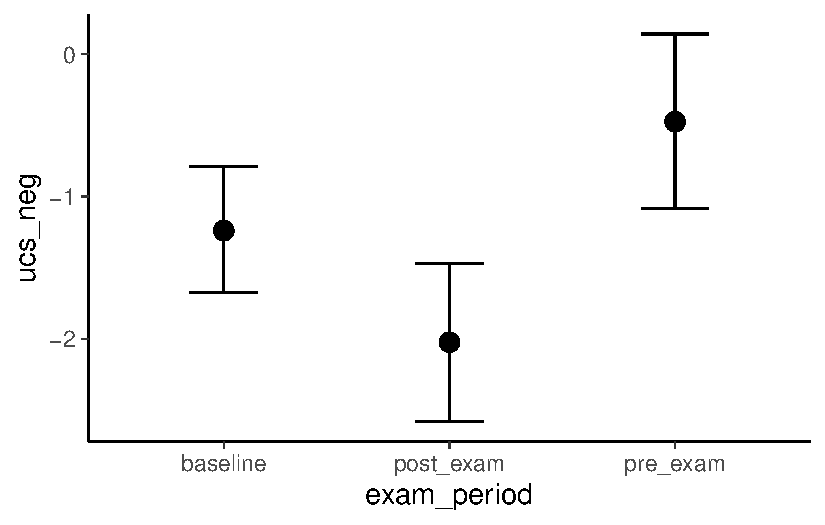
\includegraphics[keepaspectratio]{risk_files/figure-pdf/unnamed-chunk-22-1.pdf}}

\begin{Shaded}
\begin{Highlighting}[]
\FunctionTok{tapply}\NormalTok{(df\_exam\_tagged}\SpecialCharTok{$}\NormalTok{ucs\_neg, df\_exam\_tagged}\SpecialCharTok{$}\NormalTok{exam\_period, mean, }\AttributeTok{na.rm =} \ConstantTok{TRUE}\NormalTok{)}
\end{Highlighting}
\end{Shaded}

\begin{verbatim}
  baseline  post_exam   pre_exam 
-1.2906692 -1.7577519  0.3602941 
\end{verbatim}

\begin{Shaded}
\begin{Highlighting}[]
\FunctionTok{tapply}\NormalTok{(df\_exam\_tagged}\SpecialCharTok{$}\NormalTok{cs\_pos, df\_exam\_tagged}\SpecialCharTok{$}\NormalTok{exam\_period, mean, }\AttributeTok{na.rm =} \ConstantTok{TRUE}\NormalTok{)}
\end{Highlighting}
\end{Shaded}

\begin{verbatim}
 baseline post_exam  pre_exam 
1.9788878 1.5717054 0.7696078 
\end{verbatim}

\begin{Shaded}
\begin{Highlighting}[]
\FunctionTok{tapply}\NormalTok{(df\_exam\_tagged}\SpecialCharTok{$}\NormalTok{neg\_aff\_ema, df\_exam\_tagged}\SpecialCharTok{$}\NormalTok{exam\_period, mean, }\AttributeTok{na.rm =} \ConstantTok{TRUE}\NormalTok{)}
\end{Highlighting}
\end{Shaded}

\begin{verbatim}
 baseline post_exam  pre_exam 
 37.19474  33.25955  42.62661 
\end{verbatim}

\begin{Shaded}
\begin{Highlighting}[]
\NormalTok{df\_with\_delta }\OtherTok{\textless{}{-}} \FunctionTok{left\_join}\NormalTok{(df\_exam\_tagged, df\_stress\_effects,  }\AttributeTok{by =} \StringTok{"user\_id"}\NormalTok{)}
\end{Highlighting}
\end{Shaded}

\begin{Shaded}
\begin{Highlighting}[]
\NormalTok{mod2 }\OtherTok{\textless{}{-}} \FunctionTok{brm}\NormalTok{(}
\NormalTok{  delta\_ucs }\SpecialCharTok{\textasciitilde{}}\NormalTok{ domain\_negative\_affect }\SpecialCharTok{+}\NormalTok{ domain\_detachment }\SpecialCharTok{+}\NormalTok{ domain\_antagonism }\SpecialCharTok{+}
\NormalTok{    domain\_disinhibition }\SpecialCharTok{+}\NormalTok{ domain\_psychoticism }\SpecialCharTok{+}
\NormalTok{    pid5\_negative\_affectivity }\SpecialCharTok{+}\NormalTok{ pid5\_detachment }\SpecialCharTok{+}\NormalTok{ pid5\_antagonism }\SpecialCharTok{+}
\NormalTok{    pid5\_disinhibition }\SpecialCharTok{+}\NormalTok{ pid5\_psychoticism }\SpecialCharTok{+}\NormalTok{ (}\DecValTok{1} \SpecialCharTok{|}\NormalTok{ user\_id}\SpecialCharTok{/}\NormalTok{day),}
  \AttributeTok{data =}\NormalTok{ df\_with\_delta,}
  \AttributeTok{family =} \FunctionTok{gaussian}\NormalTok{(),}
  \AttributeTok{backend =} \StringTok{"cmdstanr"}\NormalTok{,}
  \AttributeTok{algorithm =} \StringTok{"meanfield"}\NormalTok{,}
  \AttributeTok{seed =} \DecValTok{123}
\NormalTok{)}
\end{Highlighting}
\end{Shaded}

\begin{Shaded}
\begin{Highlighting}[]
\FunctionTok{summary}\NormalTok{(mod2)}
\end{Highlighting}
\end{Shaded}

\begin{verbatim}
 Family: gaussian 
  Links: mu = identity; sigma = identity 
Formula: delta_ucs ~ domain_negative_affect + domain_detachment + domain_antagonism + domain_disinhibition + domain_psychoticism + pid5_negative_affectivity + pid5_detachment + pid5_antagonism + pid5_disinhibition + pid5_psychoticism + (1 | user_id/day) 
   Data: df_with_delta (Number of observations: 3397) 
  Draws: 1 chains, each with iter = 1000; warmup = 0; thin = 1;
         total post-warmup draws = 1000

Multilevel Hyperparameters:
~user_id (Number of levels: 122) 
              Estimate Est.Error l-95% CI u-95% CI Rhat Bulk_ESS Tail_ESS
sd(Intercept)     2.72      0.01     2.71     2.73 1.01      914      699

~user_id:day (Number of levels: 3138) 
              Estimate Est.Error l-95% CI u-95% CI Rhat Bulk_ESS Tail_ESS
sd(Intercept)     0.01      0.01     0.00     0.02 1.00     1088      916

Regression Coefficients:
                          Estimate Est.Error l-95% CI u-95% CI Rhat Bulk_ESS
Intercept                     2.74      0.06     2.61     2.87 1.00      940
domain_negative_affect       -0.05      0.00    -0.05    -0.04 1.00      909
domain_detachment             0.03      0.00     0.02     0.03 1.00      880
domain_antagonism            -0.05      0.00    -0.06    -0.05 1.00     1027
domain_disinhibition         -0.03      0.00    -0.03    -0.03 1.00      947
domain_psychoticism          -0.01      0.00    -0.01    -0.00 1.00     1003
pid5_negative_affectivity    -0.00      0.01    -0.01     0.01 1.00      971
pid5_detachment              -0.00      0.00    -0.01     0.01 1.00      914
pid5_antagonism              -0.01      0.01    -0.02     0.00 1.00     1008
pid5_disinhibition           -0.00      0.01    -0.02     0.02 1.00      870
pid5_psychoticism             0.00      0.01    -0.01     0.02 1.00     1010
                          Tail_ESS
Intercept                      983
domain_negative_affect         912
domain_detachment              696
domain_antagonism             1058
domain_disinhibition           975
domain_psychoticism            906
pid5_negative_affectivity      875
pid5_detachment                845
pid5_antagonism                884
pid5_disinhibition             992
pid5_psychoticism              981

Further Distributional Parameters:
      Estimate Est.Error l-95% CI u-95% CI Rhat Bulk_ESS Tail_ESS
sigma     0.54      0.01     0.52     0.56 1.00      946      944

Draws were sampled using variational(meanfield). 
\end{verbatim}

\subsection{Reattività individuale allo stress
(delta)}\label{reattivituxe0-individuale-allo-stress-delta}

\begin{Shaded}
\begin{Highlighting}[]
\CommentTok{\# Calcola cambiamenti tra baseline e post\_exam per UCS, CS, umore}
\NormalTok{df\_stress\_profile }\OtherTok{\textless{}{-}}\NormalTok{ df\_exam\_tagged }\SpecialCharTok{\%\textgreater{}\%}
\NormalTok{  dplyr}\SpecialCharTok{::}\FunctionTok{filter}\NormalTok{(exam\_period }\SpecialCharTok{\%in\%} \FunctionTok{c}\NormalTok{(}\StringTok{"baseline"}\NormalTok{, }\StringTok{"pre\_exam"}\NormalTok{, }\StringTok{"post\_exam"}\NormalTok{)) }\SpecialCharTok{\%\textgreater{}\%}
  \FunctionTok{group\_by}\NormalTok{(user\_id, exam\_period) }\SpecialCharTok{\%\textgreater{}\%}
  \FunctionTok{summarise}\NormalTok{(}
    \AttributeTok{ucs =} \FunctionTok{mean}\NormalTok{(ucs\_neg, }\AttributeTok{na.rm =} \ConstantTok{TRUE}\NormalTok{),}
    \AttributeTok{cs  =} \FunctionTok{mean}\NormalTok{(cs\_pos, }\AttributeTok{na.rm =} \ConstantTok{TRUE}\NormalTok{),}
    \AttributeTok{mood =} \FunctionTok{mean}\NormalTok{(neg\_aff\_ema, }\AttributeTok{na.rm =} \ConstantTok{TRUE}\NormalTok{),}
    \AttributeTok{.groups =} \StringTok{"drop"}
\NormalTok{  ) }\SpecialCharTok{\%\textgreater{}\%}
  \FunctionTok{pivot\_wider}\NormalTok{(}\AttributeTok{names\_from =}\NormalTok{ exam\_period, }\AttributeTok{values\_from =} \FunctionTok{c}\NormalTok{(ucs, cs, mood)) }\SpecialCharTok{\%\textgreater{}\%}
  \FunctionTok{mutate}\NormalTok{(}
    \AttributeTok{delta\_ucs  =}\NormalTok{ ucs\_post\_exam }\SpecialCharTok{{-}}\NormalTok{ ucs\_baseline,}
    \AttributeTok{delta\_cs   =}\NormalTok{ cs\_post\_exam  }\SpecialCharTok{{-}}\NormalTok{ cs\_baseline,}
    \AttributeTok{delta\_mood =}\NormalTok{ mood\_post\_exam }\SpecialCharTok{{-}}\NormalTok{ mood\_baseline,}
    
    \CommentTok{\# Opzionale: anche pre\_exam}
    \AttributeTok{delta\_ucs\_pre  =}\NormalTok{ ucs\_pre\_exam }\SpecialCharTok{{-}}\NormalTok{ ucs\_baseline,}
    \AttributeTok{delta\_cs\_pre   =}\NormalTok{ cs\_pre\_exam  }\SpecialCharTok{{-}}\NormalTok{ cs\_baseline,}
    \AttributeTok{delta\_mood\_pre =}\NormalTok{ mood\_pre\_exam }\SpecialCharTok{{-}}\NormalTok{ mood\_baseline}
\NormalTok{  )}
\end{Highlighting}
\end{Shaded}

Costruzione indice composito \texttt{stress\_reactivity}.

\begin{Shaded}
\begin{Highlighting}[]
\NormalTok{df\_stress\_profile }\OtherTok{\textless{}{-}}\NormalTok{ df\_stress\_profile }\SpecialCharTok{\%\textgreater{}\%}
  \FunctionTok{mutate}\NormalTok{(}
    \AttributeTok{z\_delta\_ucs  =} \FunctionTok{scale}\NormalTok{(delta\_ucs)[,}\DecValTok{1}\NormalTok{],}
    \AttributeTok{z\_delta\_cs   =} \FunctionTok{scale}\NormalTok{(}\SpecialCharTok{{-}}\NormalTok{delta\_cs)[,}\DecValTok{1}\NormalTok{],     }\CommentTok{\# notare il "{-}" → calo della cs = peggioramento}
    \AttributeTok{z\_delta\_mood =} \FunctionTok{scale}\NormalTok{(delta\_mood)[,}\DecValTok{1}\NormalTok{]}
\NormalTok{  ) }\SpecialCharTok{\%\textgreater{}\%}
  \FunctionTok{mutate}\NormalTok{(}
    \AttributeTok{stress\_reactivity =}\NormalTok{ z\_delta\_ucs }\SpecialCharTok{+}\NormalTok{ z\_delta\_cs }\SpecialCharTok{+}\NormalTok{ z\_delta\_mood}
\NormalTok{  )}
\end{Highlighting}
\end{Shaded}

\begin{Shaded}
\begin{Highlighting}[]
\FunctionTok{hist}\NormalTok{(df\_stress\_profile}\SpecialCharTok{$}\NormalTok{stress\_reactivity)}
\end{Highlighting}
\end{Shaded}

\pandocbounded{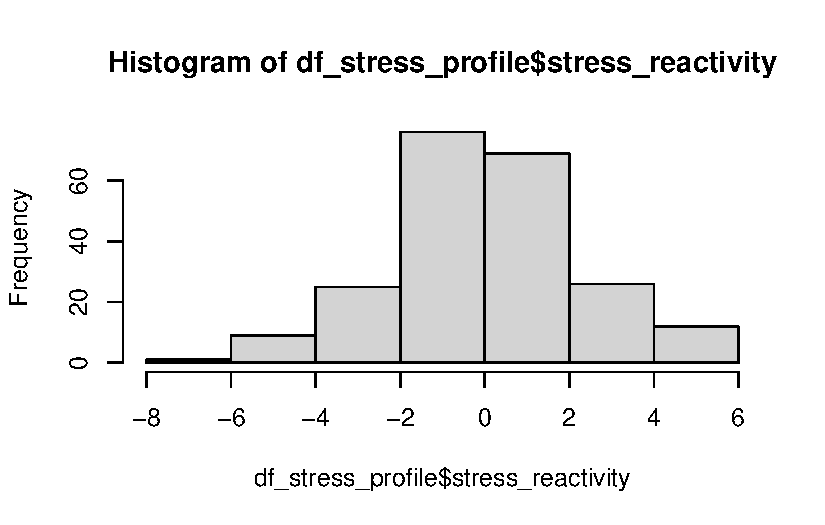
\includegraphics[keepaspectratio]{risk_files/figure-pdf/unnamed-chunk-31-1.pdf}}

\begin{Shaded}
\begin{Highlighting}[]
\NormalTok{df\_stress\_profile }\OtherTok{\textless{}{-}}\NormalTok{ df\_stress\_profile }\SpecialCharTok{\%\textgreater{}\%}
  \FunctionTok{mutate}\NormalTok{(}
    \AttributeTok{ucs\_baseline\_z =} \FunctionTok{scale}\NormalTok{(ucs\_baseline)[,}\DecValTok{1}\NormalTok{],}
    \AttributeTok{cs\_baseline\_z  =} \FunctionTok{scale}\NormalTok{(cs\_baseline)[,}\DecValTok{1}\NormalTok{],}
    \AttributeTok{mood\_baseline\_z =} \FunctionTok{scale}\NormalTok{(mood\_baseline)[,}\DecValTok{1}\NormalTok{]}
\NormalTok{  )}
\end{Highlighting}
\end{Shaded}

\begin{Shaded}
\begin{Highlighting}[]
\NormalTok{fm }\OtherTok{\textless{}{-}} \FunctionTok{lm}\NormalTok{(}
\NormalTok{  stress\_reactivity }\SpecialCharTok{\textasciitilde{}}\NormalTok{ ucs\_baseline\_z }\SpecialCharTok{+}\NormalTok{ cs\_baseline\_z }\SpecialCharTok{+}\NormalTok{ mood\_baseline\_z, }
  \AttributeTok{data =}\NormalTok{ df\_stress\_profile)}
\end{Highlighting}
\end{Shaded}

\begin{Shaded}
\begin{Highlighting}[]
\CommentTok{\# 1. Seleziona solo le colonne rilevanti e rimuovi i casi incompleti}
\NormalTok{df\_for\_pca }\OtherTok{\textless{}{-}}\NormalTok{ df\_stress\_profile }\SpecialCharTok{\%\textgreater{}\%}
\NormalTok{  dplyr}\SpecialCharTok{::}\FunctionTok{select}\NormalTok{(user\_id, z\_delta\_ucs, z\_delta\_cs, z\_delta\_mood) }\SpecialCharTok{\%\textgreater{}\%}
  \FunctionTok{drop\_na}\NormalTok{()}

\CommentTok{\# 2. Applica PCA senza ulteriori scaling (le variabili sono già standardizzate)}
\NormalTok{react\_pca }\OtherTok{\textless{}{-}} \FunctionTok{prcomp}\NormalTok{(df\_for\_pca }\SpecialCharTok{\%\textgreater{}\%}\NormalTok{ dplyr}\SpecialCharTok{::}\FunctionTok{select}\NormalTok{(}\SpecialCharTok{{-}}\NormalTok{user\_id), }\AttributeTok{scale. =} \ConstantTok{FALSE}\NormalTok{)}

\CommentTok{\# 3. Aggiungi il primo componente al dataframe}
\NormalTok{df\_for\_pca }\OtherTok{\textless{}{-}}\NormalTok{ df\_for\_pca }\SpecialCharTok{\%\textgreater{}\%}
  \FunctionTok{mutate}\NormalTok{(}\AttributeTok{stress\_reactivity\_pca =}\NormalTok{ react\_pca}\SpecialCharTok{$}\NormalTok{x[, }\DecValTok{1}\NormalTok{])}
\end{Highlighting}
\end{Shaded}

\begin{Shaded}
\begin{Highlighting}[]
\NormalTok{df\_stress\_profile }\OtherTok{\textless{}{-}}\NormalTok{ df\_stress\_profile }\SpecialCharTok{\%\textgreater{}\%}
  \FunctionTok{left\_join}\NormalTok{(df\_for\_pca }\SpecialCharTok{\%\textgreater{}\%}\NormalTok{ dplyr}\SpecialCharTok{::}\FunctionTok{select}\NormalTok{(user\_id, stress\_reactivity\_pca), }\AttributeTok{by =} \StringTok{"user\_id"}\NormalTok{)}
\end{Highlighting}
\end{Shaded}

\begin{Shaded}
\begin{Highlighting}[]
\NormalTok{pid5\_baseline }\OtherTok{\textless{}{-}}\NormalTok{ df\_exam\_tagged }\SpecialCharTok{|\textgreater{}} 
\NormalTok{  dplyr}\SpecialCharTok{::}\FunctionTok{select}\NormalTok{(}
\NormalTok{    user\_id, domain\_negative\_affect, domain\_detachment, domain\_antagonism,}
\NormalTok{    domain\_disinhibition, domain\_psychoticism}
\NormalTok{  ) }\SpecialCharTok{|\textgreater{}} 
\NormalTok{  dplyr}\SpecialCharTok{::}\FunctionTok{distinct}\NormalTok{(user\_id, }\AttributeTok{.keep\_all =} \ConstantTok{TRUE}\NormalTok{)}
\end{Highlighting}
\end{Shaded}

\begin{Shaded}
\begin{Highlighting}[]
\NormalTok{df }\OtherTok{\textless{}{-}} \FunctionTok{left\_join}\NormalTok{(df\_stress\_profile, pid5\_baseline, }\AttributeTok{by =} \StringTok{"user\_id"}\NormalTok{) }
\end{Highlighting}
\end{Shaded}

\subsection{Regressioni lineari: baseline e tratti
EMA}\label{regressioni-lineari-baseline-e-tratti-ema}

\begin{Shaded}
\begin{Highlighting}[]
\CommentTok{\# Regressione su tratti basali PID{-}5}
\NormalTok{model\_pid5 }\OtherTok{\textless{}{-}} \FunctionTok{lm}\NormalTok{(}
\NormalTok{  stress\_reactivity\_pca }\SpecialCharTok{\textasciitilde{}} 
\NormalTok{    domain\_negative\_affect }\SpecialCharTok{+}
\NormalTok{    domain\_detachment }\SpecialCharTok{+}
\NormalTok{    domain\_antagonism }\SpecialCharTok{+}
\NormalTok{    domain\_disinhibition }\SpecialCharTok{+}
\NormalTok{    domain\_psychoticism,}
  \AttributeTok{data =}\NormalTok{ df}
\NormalTok{)}
\end{Highlighting}
\end{Shaded}

\begin{Shaded}
\begin{Highlighting}[]
\FunctionTok{summary}\NormalTok{(model\_pid5)}
\end{Highlighting}
\end{Shaded}

\begin{verbatim}

Call:
lm(formula = stress_reactivity_pca ~ domain_negative_affect + 
    domain_detachment + domain_antagonism + domain_disinhibition + 
    domain_psychoticism, data = df)

Residuals:
    Min      1Q  Median      3Q     Max 
-4.0359 -0.7356 -0.0681  0.7739  3.5420 

Coefficients:
                        Estimate Std. Error t value Pr(>|t|)
(Intercept)             0.372445   0.291446   1.278    0.203
domain_negative_affect -0.004138   0.009067  -0.456    0.649
domain_detachment      -0.018050   0.011067  -1.631    0.104
domain_antagonism       0.002868   0.012071   0.238    0.812
domain_disinhibition    0.009874   0.012574   0.785    0.433
domain_psychoticism    -0.006733   0.007770  -0.867    0.387

Residual standard error: 1.346 on 199 degrees of freedom
  (174 observations deleted due to missingness)
Multiple R-squared:  0.02829,   Adjusted R-squared:  0.003873 
F-statistic: 1.159 on 5 and 199 DF,  p-value: 0.331
\end{verbatim}

\begin{Shaded}
\begin{Highlighting}[]
\NormalTok{df2\_augmented }\OtherTok{\textless{}{-}}\NormalTok{ df2 }\SpecialCharTok{\%\textgreater{}\%}
  \FunctionTok{left\_join}\NormalTok{(}
\NormalTok{    df\_stress\_profile }\SpecialCharTok{\%\textgreater{}\%}\NormalTok{ dplyr}\SpecialCharTok{::}\FunctionTok{select}\NormalTok{(user\_id, stress\_reactivity\_pca),}
    \AttributeTok{by =} \StringTok{"user\_id"}
\NormalTok{  )}
\end{Highlighting}
\end{Shaded}

\begin{Shaded}
\begin{Highlighting}[]
\CommentTok{\# Modello bayesiano con effetti casuali per soggetto}
\NormalTok{mod\_aug }\OtherTok{\textless{}{-}} \FunctionTok{brm}\NormalTok{(}
\NormalTok{  stress\_reactivity\_pca }\SpecialCharTok{\textasciitilde{}}
\NormalTok{    pid5\_negative\_affectivity }\SpecialCharTok{+}\NormalTok{ pid5\_detachment }\SpecialCharTok{+}\NormalTok{ pid5\_antagonism }\SpecialCharTok{+}
\NormalTok{    pid5\_disinhibition }\SpecialCharTok{+}\NormalTok{ pid5\_psychoticism }\SpecialCharTok{+}
\NormalTok{    (}\DecValTok{1} \SpecialCharTok{+}\NormalTok{ pid5\_negative\_affectivity }\SpecialCharTok{+}\NormalTok{ pid5\_detachment }\SpecialCharTok{+}\NormalTok{ pid5\_antagonism }\SpecialCharTok{+}
\NormalTok{       pid5\_disinhibition }\SpecialCharTok{+}\NormalTok{ pid5\_psychoticism }\SpecialCharTok{|}\NormalTok{ user\_id}\SpecialCharTok{/}\NormalTok{day),}
  \AttributeTok{data =}\NormalTok{ df2\_augmented,}
  \AttributeTok{family =} \FunctionTok{gaussian}\NormalTok{(),}
  \AttributeTok{backend =} \StringTok{"cmdstanr"}\NormalTok{,}
  \AttributeTok{algorithm =} \StringTok{"meanfield"}\NormalTok{,}
  \AttributeTok{seed =} \DecValTok{123}
\NormalTok{)}
\end{Highlighting}
\end{Shaded}

\begin{Shaded}
\begin{Highlighting}[]
\FunctionTok{summary}\NormalTok{(mod\_aug)}
\end{Highlighting}
\end{Shaded}

\begin{verbatim}
 Family: gaussian 
  Links: mu = identity; sigma = identity 
Formula: stress_reactivity_pca ~ pid5_negative_affectivity + pid5_detachment + pid5_antagonism + pid5_disinhibition + pid5_psychoticism + (1 + pid5_negative_affectivity + pid5_detachment + pid5_antagonism + pid5_disinhibition + pid5_psychoticism | user_id/day) 
   Data: df2_augmented (Number of observations: 5880) 
  Draws: 1 chains, each with iter = 1000; warmup = 0; thin = 1;
         total post-warmup draws = 1000

Multilevel Hyperparameters:
~user_id (Number of levels: 218) 
                                                  Estimate Est.Error l-95% CI
sd(Intercept)                                         0.28      0.17     0.08
sd(pid5_negative_affectivity)                         0.21      0.02     0.18
sd(pid5_detachment)                                   0.05      0.01     0.03
sd(pid5_antagonism)                                   0.20      0.03     0.15
sd(pid5_disinhibition)                                0.23      0.02     0.18
sd(pid5_psychoticism)                                 0.25      0.03     0.20
cor(Intercept,pid5_negative_affectivity)              0.98      0.00     0.97
cor(Intercept,pid5_detachment)                        0.87      0.13     0.49
cor(pid5_negative_affectivity,pid5_detachment)        0.82      0.14     0.43
cor(Intercept,pid5_antagonism)                        0.98      0.01     0.95
cor(pid5_negative_affectivity,pid5_antagonism)        0.95      0.02     0.90
cor(pid5_detachment,pid5_antagonism)                  0.83      0.14     0.46
cor(Intercept,pid5_disinhibition)                     1.00      0.00     0.99
cor(pid5_negative_affectivity,pid5_disinhibition)     0.97      0.01     0.95
cor(pid5_detachment,pid5_disinhibition)               0.87      0.13     0.51
cor(pid5_antagonism,pid5_disinhibition)               0.98      0.01     0.95
cor(Intercept,pid5_psychoticism)                     -0.97      0.01    -0.99
cor(pid5_negative_affectivity,pid5_psychoticism)     -0.99      0.01    -0.99
cor(pid5_detachment,pid5_psychoticism)               -0.77      0.16    -0.94
cor(pid5_antagonism,pid5_psychoticism)               -0.96      0.02    -0.99
cor(pid5_disinhibition,pid5_psychoticism)            -0.96      0.01    -0.98
                                                  u-95% CI Rhat Bulk_ESS
sd(Intercept)                                         0.71 1.00      952
sd(pid5_negative_affectivity)                         0.24 1.00      951
sd(pid5_detachment)                                   0.08 1.00      901
sd(pid5_antagonism)                                   0.25 1.00      993
sd(pid5_disinhibition)                                0.28 1.00      851
sd(pid5_psychoticism)                                 0.30 1.00      931
cor(Intercept,pid5_negative_affectivity)              0.99 1.00      975
cor(Intercept,pid5_detachment)                        0.99 1.00      954
cor(pid5_negative_affectivity,pid5_detachment)        0.97 1.00      991
cor(Intercept,pid5_antagonism)                        1.00 1.00      883
cor(pid5_negative_affectivity,pid5_antagonism)        0.98 1.00      872
cor(pid5_detachment,pid5_antagonism)                  0.97 1.00      970
cor(Intercept,pid5_disinhibition)                     1.00 1.00      898
cor(pid5_negative_affectivity,pid5_disinhibition)     0.99 1.00     1069
cor(pid5_detachment,pid5_disinhibition)               0.99 1.00      936
cor(pid5_antagonism,pid5_disinhibition)               1.00 1.00      958
cor(Intercept,pid5_psychoticism)                     -0.95 1.00      809
cor(pid5_negative_affectivity,pid5_psychoticism)     -0.97 1.00      998
cor(pid5_detachment,pid5_psychoticism)               -0.33 1.00      945
cor(pid5_antagonism,pid5_psychoticism)               -0.91 1.00      891
cor(pid5_disinhibition,pid5_psychoticism)            -0.93 1.00      872
                                                  Tail_ESS
sd(Intercept)                                          840
sd(pid5_negative_affectivity)                          901
sd(pid5_detachment)                                    879
sd(pid5_antagonism)                                    937
sd(pid5_disinhibition)                                 801
sd(pid5_psychoticism)                                  788
cor(Intercept,pid5_negative_affectivity)               899
cor(Intercept,pid5_detachment)                         944
cor(pid5_negative_affectivity,pid5_detachment)         908
cor(Intercept,pid5_antagonism)                         891
cor(pid5_negative_affectivity,pid5_antagonism)         881
cor(pid5_detachment,pid5_antagonism)                   900
cor(Intercept,pid5_disinhibition)                      979
cor(pid5_negative_affectivity,pid5_disinhibition)     1026
cor(pid5_detachment,pid5_disinhibition)                712
cor(pid5_antagonism,pid5_disinhibition)                869
cor(Intercept,pid5_psychoticism)                      1062
cor(pid5_negative_affectivity,pid5_psychoticism)       983
cor(pid5_detachment,pid5_psychoticism)                 844
cor(pid5_antagonism,pid5_psychoticism)                 944
cor(pid5_disinhibition,pid5_psychoticism)              696

~user_id:day (Number of levels: 5471) 
                                                  Estimate Est.Error l-95% CI
sd(Intercept)                                         0.05      0.01     0.03
sd(pid5_negative_affectivity)                         0.10      0.01     0.09
sd(pid5_detachment)                                   0.17      0.01     0.15
sd(pid5_antagonism)                                   0.09      0.01     0.07
sd(pid5_disinhibition)                                0.05      0.01     0.03
sd(pid5_psychoticism)                                 0.07      0.01     0.05
cor(Intercept,pid5_negative_affectivity)              1.00      0.00     0.99
cor(Intercept,pid5_detachment)                       -1.00      0.00    -1.00
cor(pid5_negative_affectivity,pid5_detachment)       -0.99      0.00    -1.00
cor(Intercept,pid5_antagonism)                       -0.99      0.01    -1.00
cor(pid5_negative_affectivity,pid5_antagonism)       -0.99      0.01    -1.00
cor(pid5_detachment,pid5_antagonism)                  0.99      0.01     0.96
cor(Intercept,pid5_disinhibition)                    -0.89      0.07    -0.97
cor(pid5_negative_affectivity,pid5_disinhibition)    -0.92      0.06    -0.99
cor(pid5_detachment,pid5_disinhibition)               0.88      0.07     0.71
cor(pid5_antagonism,pid5_disinhibition)               0.88      0.07     0.71
cor(Intercept,pid5_psychoticism)                      0.99      0.01     0.96
cor(pid5_negative_affectivity,pid5_psychoticism)      0.99      0.01     0.97
cor(pid5_detachment,pid5_psychoticism)               -0.99      0.01    -1.00
cor(pid5_antagonism,pid5_psychoticism)               -0.98      0.02    -1.00
cor(pid5_disinhibition,pid5_psychoticism)            -0.91      0.07    -0.98
                                                  u-95% CI Rhat Bulk_ESS
sd(Intercept)                                         0.08 1.00     1042
sd(pid5_negative_affectivity)                         0.12 1.00      895
sd(pid5_detachment)                                   0.19 1.01      886
sd(pid5_antagonism)                                   0.12 1.00     1082
sd(pid5_disinhibition)                                0.07 1.00     1003
sd(pid5_psychoticism)                                 0.10 1.00     1007
cor(Intercept,pid5_negative_affectivity)              1.00 1.00      999
cor(Intercept,pid5_detachment)                       -1.00 1.00     1004
cor(pid5_negative_affectivity,pid5_detachment)       -0.99 1.00     1026
cor(Intercept,pid5_antagonism)                       -0.97 1.00     1008
cor(pid5_negative_affectivity,pid5_antagonism)       -0.96 1.00     1020
cor(pid5_detachment,pid5_antagonism)                  1.00 1.00     1026
cor(Intercept,pid5_disinhibition)                    -0.73 1.00      959
cor(pid5_negative_affectivity,pid5_disinhibition)    -0.78 1.00      952
cor(pid5_detachment,pid5_disinhibition)               0.96 1.00      953
cor(pid5_antagonism,pid5_disinhibition)               0.97 1.00      939
cor(Intercept,pid5_psychoticism)                      1.00 1.00      896
cor(pid5_negative_affectivity,pid5_psychoticism)      1.00 1.00     1038
cor(pid5_detachment,pid5_psychoticism)               -0.95 1.00      881
cor(pid5_antagonism,pid5_psychoticism)               -0.94 1.00      832
cor(pid5_disinhibition,pid5_psychoticism)            -0.73 1.00     1031
                                                  Tail_ESS
sd(Intercept)                                         1024
sd(pid5_negative_affectivity)                          801
sd(pid5_detachment)                                    982
sd(pid5_antagonism)                                    876
sd(pid5_disinhibition)                                 876
sd(pid5_psychoticism)                                  906
cor(Intercept,pid5_negative_affectivity)               834
cor(Intercept,pid5_detachment)                         983
cor(pid5_negative_affectivity,pid5_detachment)         914
cor(Intercept,pid5_antagonism)                         875
cor(pid5_negative_affectivity,pid5_antagonism)         944
cor(pid5_detachment,pid5_antagonism)                   759
cor(Intercept,pid5_disinhibition)                      901
cor(pid5_negative_affectivity,pid5_disinhibition)      947
cor(pid5_detachment,pid5_disinhibition)                944
cor(pid5_antagonism,pid5_disinhibition)                944
cor(Intercept,pid5_psychoticism)                       908
cor(pid5_negative_affectivity,pid5_psychoticism)       988
cor(pid5_detachment,pid5_psychoticism)                 981
cor(pid5_antagonism,pid5_psychoticism)                 983
cor(pid5_disinhibition,pid5_psychoticism)             1026

Regression Coefficients:
                          Estimate Est.Error l-95% CI u-95% CI Rhat Bulk_ESS
Intercept                     0.01      0.21    -0.35     0.42 1.00      728
pid5_negative_affectivity     0.00      0.04    -0.06     0.07 1.00      805
pid5_detachment               0.04      0.03    -0.03     0.10 1.00      978
pid5_antagonism               0.04      0.05    -0.06     0.13 1.00      845
pid5_disinhibition           -0.00      0.04    -0.08     0.07 1.00      925
pid5_psychoticism            -0.05      0.05    -0.14     0.05 1.00      912
                          Tail_ESS
Intercept                      796
pid5_negative_affectivity      863
pid5_detachment                943
pid5_antagonism                843
pid5_disinhibition             850
pid5_psychoticism              981

Further Distributional Parameters:
      Estimate Est.Error l-95% CI u-95% CI Rhat Bulk_ESS Tail_ESS
sigma     0.57      0.03     0.52     0.62 1.00      755      841

Draws were sampled using variational(meanfield). 
\end{verbatim}

Questa analisi non dice niente di interessante.

\subsection{Analisi della variabilità dei tratti
EMA}\label{analisi-della-variabilituxe0-dei-tratti-ema}

\begin{Shaded}
\begin{Highlighting}[]
\CommentTok{\# Calcola la deviazione standard dei tratti EMA per soggetto}
\NormalTok{pid5\_variability }\OtherTok{\textless{}{-}}\NormalTok{ df2 }\SpecialCharTok{\%\textgreater{}\%}
  \FunctionTok{group\_by}\NormalTok{(user\_id) }\SpecialCharTok{\%\textgreater{}\%}
  \FunctionTok{summarise}\NormalTok{(}
    \AttributeTok{sd\_neg\_aff =} \FunctionTok{sd}\NormalTok{(pid5\_negative\_affectivity, }\AttributeTok{na.rm =} \ConstantTok{TRUE}\NormalTok{),}
    \AttributeTok{sd\_detach  =} \FunctionTok{sd}\NormalTok{(pid5\_detachment, }\AttributeTok{na.rm =} \ConstantTok{TRUE}\NormalTok{),}
    \AttributeTok{sd\_antag   =} \FunctionTok{sd}\NormalTok{(pid5\_antagonism, }\AttributeTok{na.rm =} \ConstantTok{TRUE}\NormalTok{),}
    \AttributeTok{sd\_disinh  =} \FunctionTok{sd}\NormalTok{(pid5\_disinhibition, }\AttributeTok{na.rm =} \ConstantTok{TRUE}\NormalTok{),}
    \AttributeTok{sd\_psych   =} \FunctionTok{sd}\NormalTok{(pid5\_psychoticism, }\AttributeTok{na.rm =} \ConstantTok{TRUE}\NormalTok{),}
    \AttributeTok{.groups =} \StringTok{"drop"}
\NormalTok{  )}

\CommentTok{\# 2. Merge with the stress reactivity PCA measure}
\NormalTok{pid5\_variability }\OtherTok{\textless{}{-}}\NormalTok{ pid5\_variability }\SpecialCharTok{\%\textgreater{}\%}
  \FunctionTok{left\_join}\NormalTok{(}
\NormalTok{    df\_stress\_profile }\SpecialCharTok{\%\textgreater{}\%}\NormalTok{ dplyr}\SpecialCharTok{::}\FunctionTok{select}\NormalTok{(user\_id, stress\_reactivity\_pca),}
    \AttributeTok{by =} \StringTok{"user\_id"}
\NormalTok{  )}

\CommentTok{\# 3. Fit the linear model}
\NormalTok{fm }\OtherTok{\textless{}{-}} \FunctionTok{lm}\NormalTok{(}
\NormalTok{  stress\_reactivity\_pca }\SpecialCharTok{\textasciitilde{}}\NormalTok{ sd\_neg\_aff }\SpecialCharTok{+}\NormalTok{ sd\_detach }\SpecialCharTok{+}\NormalTok{ sd\_antag }\SpecialCharTok{+}\NormalTok{ sd\_disinh }\SpecialCharTok{+}\NormalTok{ sd\_psych, }
  \AttributeTok{data =}\NormalTok{ pid5\_variability}
\NormalTok{)}

\CommentTok{\# 4. View summary}
\FunctionTok{summary}\NormalTok{(fm)}
\end{Highlighting}
\end{Shaded}

\begin{verbatim}

Call:
lm(formula = stress_reactivity_pca ~ sd_neg_aff + sd_detach + 
    sd_antag + sd_disinh + sd_psych, data = pid5_variability)

Residuals:
    Min      1Q  Median      3Q     Max 
-4.3914 -0.7179 -0.1004  0.7152  3.6946 

Coefficients:
            Estimate Std. Error t value Pr(>|t|)
(Intercept)   0.3805     0.3268   1.164    0.246
sd_neg_aff   -0.1724     0.2506  -0.688    0.492
sd_detach    -0.2644     0.2061  -1.283    0.201
sd_antag      0.2506     0.1989   1.260    0.209
sd_disinh     0.1600     0.2819   0.567    0.571
sd_psych     -0.2538     0.1844  -1.376    0.170

Residual standard error: 1.331 on 212 degrees of freedom
  (161 observations deleted due to missingness)
Multiple R-squared:  0.02741,   Adjusted R-squared:  0.004477 
F-statistic: 1.195 on 5 and 212 DF,  p-value: 0.3126
\end{verbatim}

Anche in questo modo non si ottengono risultati utili.

\subsection{Full bayesian model}\label{full-bayesian-model}

\subsubsection{Contesto del Modello}\label{contesto-del-modello}

Il modello ha lo scopo di verificare se e come le \emph{variazioni
temporali intra-individuali} dei 5 domini del PID-5 (misurati tramite
EMA) siano predittive della \emph{reattività allo stress}. L'obiettivo è
mostrare che le \emph{fluttuazioni} dei tratti nel tempo (piuttosto che
una misurazione singola statica) forniscono informazioni utili sulla
vulnerabilità o adattività degli individui.

Analizziamo nel dettaglio le proprietà dei dati usati come input per il
modello bayesiano completo. Questo commento ti permette di comprendere
con precisione cosa viene analizzato e come il modello interpreta i dati
a livello sia \emph{intra-} che \emph{inter-soggettivo}.

\paragraph{Variabili EMA (input dinamico del
modello)}\label{variabili-ema-input-dinamico-del-modello}

\begin{Shaded}
\begin{Highlighting}[]
\NormalTok{ema\_vars }\OtherTok{\textless{}{-}} \FunctionTok{c}\NormalTok{(}
  \StringTok{"pid5\_negative\_affectivity"}\NormalTok{,}
  \StringTok{"pid5\_detachment"}\NormalTok{,}
  \StringTok{"pid5\_antagonism"}\NormalTok{,}
  \StringTok{"pid5\_disinhibition"}\NormalTok{,}
  \StringTok{"pid5\_psychoticism"}
\NormalTok{)}
\end{Highlighting}
\end{Shaded}

Queste sono le 5 dimensioni del modello PID-5, misurate
\emph{ripetutamente} nel tempo via EMA (Ecological Momentary
Assessment). Ogni variabile è quindi un \emph{time series} soggettiva,
che riflette come ciascun tratto si modifica nell'arco delle settimane
(tipicamente 1-2 volte a settimana per 2 mesi nello studio).

\paragraph{Pre-processing dei dati}\label{pre-processing-dei-dati}

\begin{enumerate}
\def\labelenumi{\arabic{enumi}.}
\item
  \textbf{Rimozione delle osservazioni con missing:}

\begin{Shaded}
\begin{Highlighting}[]
\NormalTok{df2 }\OtherTok{\textless{}{-}}\NormalTok{ df2 }\SpecialCharTok{\%\textgreater{}\%}\NormalTok{ dplyr}\SpecialCharTok{::}\FunctionTok{filter}\NormalTok{(}\FunctionTok{if\_all}\NormalTok{(}\FunctionTok{all\_of}\NormalTok{(ema\_vars), }\SpecialCharTok{\textasciitilde{}} \SpecialCharTok{!}\FunctionTok{is.na}\NormalTok{(.x)))}
\end{Highlighting}
\end{Shaded}

  Solo le osservazioni con dati completi sui 5 tratti vengono incluse,
  assicurando che ogni riga della matrice \texttt{y} abbia informazioni
  complete.
\item
  \textbf{Inclusione dei soli soggetti con punteggio noto di reattività
  allo stress:}

\begin{Shaded}
\begin{Highlighting}[]
\NormalTok{valid\_ids }\OtherTok{\textless{}{-}}\NormalTok{ df\_stress\_profile }\SpecialCharTok{\%\textgreater{}\%}
  \FunctionTok{filter}\NormalTok{(}\SpecialCharTok{!}\FunctionTok{is.na}\NormalTok{(stress\_reactivity\_pca)) }\SpecialCharTok{\%\textgreater{}\%}
  \FunctionTok{pull}\NormalTok{(user\_id)}
\NormalTok{df2 }\OtherTok{\textless{}{-}}\NormalTok{ df2 }\SpecialCharTok{\%\textgreater{}\%} \FunctionTok{filter}\NormalTok{(user\_id }\SpecialCharTok{\%in\%}\NormalTok{ valid\_ids)}
\end{Highlighting}
\end{Shaded}

  In questo modo si garantisce che il \emph{target} del modello
  (\texttt{stress\_reactivity\_pca}) sia disponibile per ogni soggetto
  incluso.
\item
  \textbf{Creazione dell'indice del soggetto (\texttt{subj\_idx}) e del
  tempo (\texttt{time\_idx}):}

  \begin{itemize}
  \tightlist
  \item
    Ogni soggetto riceve un indice intero univoco (1\ldots J).
  \item
    All'interno di ciascun soggetto, le osservazioni EMA vengono
    ordinate cronologicamente e numerate da 1 a Tᵢ.
  \end{itemize}

  Questo permette di modellare correttamente la dinamica latente del
  tratto nel tempo per ciascun soggetto.
\end{enumerate}

\paragraph{Dimensioni dei dati finali}\label{dimensioni-dei-dati-finali}

\begin{itemize}
\tightlist
\item
  \texttt{N}: numero totale di osservazioni EMA (righe in \texttt{df2}).
\item
  \texttt{J}: numero di soggetti.
\item
  \texttt{K\ =\ 5}: numero di tratti EMA dinamici.
\item
  \texttt{y}: matrice \(N \times K\), contenente le osservazioni EMA.
\item
  \texttt{subj\_id}: vettore di lunghezza N che assegna ogni
  osservazione EMA al suo soggetto.
\item
  \texttt{stress\_reactivity}: vettore di lunghezza J, contenente il
  punteggio target (reattività allo stress).
\item
  \texttt{N\_per}: vettore di lunghezza J che indica il numero di
  osservazioni EMA per ciascun soggetto.
\item
  \texttt{subj\_n}: matrice \(J \times \texttt{max\_N\_per}\), che
  contiene per ogni soggetto gli indici delle osservazioni
  corrispondenti (serve per calcolare la deviazione standard latente a
  livello individuale nei modelli gerarchici).
\end{itemize}

\paragraph{Cosa analizza esattamente il
modello}\label{cosa-analizza-esattamente-il-modello}

Per ciascun tratto \(k \in 1..5\), e per ciascun soggetto \(j\), il
modello stima una \textbf{serie latente \(\theta\_{k}(t)\)} che evolve
nel tempo secondo un processo stocastico (random walk o AR(1), nel tuo
caso un RW semplice):

\[
\theta_{k}(t) \sim \mathcal{N}(\theta_{k}(t-1), \sigma_{\theta_k})
\]

Questa latente viene poi confrontata con i dati osservati tramite una
likelihood gaussiana:

\[
y_{n,k} \sim \mathcal{N}(\theta_{k}(n), \sigma_{y_k})
\]

Infine, si calcola per ogni soggetto la \textbf{deviazione standard} dei
valori latenti per ciascun tratto, cioè quanto il tratto varia nel tempo
per quel soggetto. Questa variabilità temporale è poi usata per predire:

\[
\texttt{stress\_reactivity}_j \sim \mathcal{N}(\alpha + \beta_1 \cdot \texttt{SD}_{j,1} + \cdots + \beta_5 \cdot \texttt{SD}_{j,5}, \sigma_r)
\]

\paragraph{In sintesi}\label{in-sintesi}

Il modello:

\begin{itemize}
\tightlist
\item
  non si limita a medie statiche dei tratti,
\item
  non aggrega le misure EMA per soggetto,
\item
  ma stima una \textbf{dinamica latente individuale} per ogni tratto →
  calcola \textbf{quanto ciascun tratto fluttua} nel tempo per ciascun
  soggetto,
\item
  e verifica \textbf{se questa fluttuazione è predittiva della
  reattività allo stress}.
\end{itemize}

Questa scelta metodologica è in linea con l'ipotesi centrale dello
studio: le \textbf{dinamiche intra-individuali} dei tratti sono
informative e potenzialmente più predittive rispetto alle sole misure
statiche.

\begin{Shaded}
\begin{Highlighting}[]
\NormalTok{ema\_vars }\OtherTok{\textless{}{-}} \FunctionTok{c}\NormalTok{(}
  \StringTok{"pid5\_negative\_affectivity"}\NormalTok{,}
  \StringTok{"pid5\_detachment"}\NormalTok{,}
  \StringTok{"pid5\_antagonism"}\NormalTok{,}
  \StringTok{"pid5\_disinhibition"}\NormalTok{,}
  \StringTok{"pid5\_psychoticism"}
\NormalTok{)}

\CommentTok{\# Remove rows with missing EMA traits}
\NormalTok{df2 }\OtherTok{\textless{}{-}}\NormalTok{ df2 }\SpecialCharTok{\%\textgreater{}\%} 
\NormalTok{  dplyr}\SpecialCharTok{::}\FunctionTok{filter}\NormalTok{(}\FunctionTok{if\_all}\NormalTok{(}\FunctionTok{all\_of}\NormalTok{(ema\_vars), }\SpecialCharTok{\textasciitilde{}} \SpecialCharTok{!}\FunctionTok{is.na}\NormalTok{(.x)))}

\CommentTok{\# Create integer subject index}
\NormalTok{df2 }\OtherTok{\textless{}{-}}\NormalTok{ df2 }\SpecialCharTok{\%\textgreater{}\%}
\NormalTok{  dplyr}\SpecialCharTok{::}\FunctionTok{filter}\NormalTok{(}\SpecialCharTok{!}\FunctionTok{is.na}\NormalTok{(user\_id)) }\SpecialCharTok{\%\textgreater{}\%}
  \FunctionTok{mutate}\NormalTok{(}\AttributeTok{user\_idx =} \FunctionTok{as.integer}\NormalTok{(}\FunctionTok{factor}\NormalTok{(user\_id)))}

\CommentTok{\# Keep only subjects with non{-}missing stress reactivity}
\NormalTok{valid\_ids }\OtherTok{\textless{}{-}}\NormalTok{ df\_stress\_profile }\SpecialCharTok{\%\textgreater{}\%}
\NormalTok{  dplyr}\SpecialCharTok{::}\FunctionTok{filter}\NormalTok{(}\SpecialCharTok{!}\FunctionTok{is.na}\NormalTok{(stress\_reactivity\_pca)) }\SpecialCharTok{\%\textgreater{}\%}
  \FunctionTok{pull}\NormalTok{(user\_id)}

\CommentTok{\# Filter df2 accordingly}
\NormalTok{df2 }\OtherTok{\textless{}{-}}\NormalTok{ df2 }\SpecialCharTok{\%\textgreater{}\%} 
\NormalTok{  dplyr}\SpecialCharTok{::}\FunctionTok{filter}\NormalTok{(user\_id }\SpecialCharTok{\%in\%}\NormalTok{ valid\_ids)}

\CommentTok{\# Recalculate subj\_idx since some subjects were dropped}
\NormalTok{df2 }\OtherTok{\textless{}{-}}\NormalTok{ df2 }\SpecialCharTok{\%\textgreater{}\%}
  \FunctionTok{mutate}\NormalTok{(}\AttributeTok{subj\_idx =} \FunctionTok{as.integer}\NormalTok{(}\FunctionTok{factor}\NormalTok{(user\_id)))}

\CommentTok{\# Also reindex time within subject}
\NormalTok{df2 }\OtherTok{\textless{}{-}}\NormalTok{ df2 }\SpecialCharTok{\%\textgreater{}\%}
  \FunctionTok{group\_by}\NormalTok{(subj\_idx) }\SpecialCharTok{\%\textgreater{}\%}
  \FunctionTok{arrange}\NormalTok{(day) }\SpecialCharTok{\%\textgreater{}\%}
  \FunctionTok{mutate}\NormalTok{(}\AttributeTok{time\_idx =} \FunctionTok{row\_number}\NormalTok{()) }\SpecialCharTok{\%\textgreater{}\%}
  \FunctionTok{ungroup}\NormalTok{()}

\CommentTok{\# Update J and N}
\NormalTok{J }\OtherTok{\textless{}{-}} \FunctionTok{length}\NormalTok{(}\FunctionTok{unique}\NormalTok{(df2}\SpecialCharTok{$}\NormalTok{subj\_idx))}
\NormalTok{N }\OtherTok{\textless{}{-}} \FunctionTok{nrow}\NormalTok{(df2)}

\CommentTok{\# Rebuild subject{-}specific indices}
\NormalTok{subj\_n }\OtherTok{\textless{}{-}} \FunctionTok{split}\NormalTok{(}\DecValTok{1}\SpecialCharTok{:}\NormalTok{N, df2}\SpecialCharTok{$}\NormalTok{subj\_idx)}
\NormalTok{N\_per }\OtherTok{\textless{}{-}} \FunctionTok{lengths}\NormalTok{(subj\_n)}
\NormalTok{max\_N\_per }\OtherTok{\textless{}{-}} \FunctionTok{max}\NormalTok{(N\_per)}

\CommentTok{\# Padded matrix of indices (J x max\_N\_per)}
\NormalTok{subj\_n\_padded }\OtherTok{\textless{}{-}} \FunctionTok{matrix}\NormalTok{(}\DecValTok{0}\NormalTok{, }\AttributeTok{nrow =}\NormalTok{ J, }\AttributeTok{ncol =}\NormalTok{ max\_N\_per)}
\ControlFlowTok{for}\NormalTok{ (j }\ControlFlowTok{in} \DecValTok{1}\SpecialCharTok{:}\NormalTok{J) \{}
\NormalTok{  subj\_n\_padded[j, }\DecValTok{1}\SpecialCharTok{:}\FunctionTok{length}\NormalTok{(subj\_n[[j]])] }\OtherTok{\textless{}{-}}\NormalTok{ subj\_n[[j]]}
\NormalTok{\}}

\CommentTok{\# Ensure alignment of outcome}
\NormalTok{df\_stress\_profile }\OtherTok{\textless{}{-}}\NormalTok{ df\_stress\_profile }\SpecialCharTok{\%\textgreater{}\%}
\NormalTok{  dplyr}\SpecialCharTok{::}\FunctionTok{filter}\NormalTok{(user\_id }\SpecialCharTok{\%in\%} \FunctionTok{unique}\NormalTok{(df2}\SpecialCharTok{$}\NormalTok{user\_id)) }\SpecialCharTok{\%\textgreater{}\%}
  \FunctionTok{arrange}\NormalTok{(}\FunctionTok{match}\NormalTok{(user\_id, }\FunctionTok{unique}\NormalTok{(df2}\SpecialCharTok{$}\NormalTok{user\_id)))  }\CommentTok{\# to ensure correct order}

\CommentTok{\# Construct Stan data}
\NormalTok{stan\_data }\OtherTok{\textless{}{-}} \FunctionTok{list}\NormalTok{(}
  \AttributeTok{N =}\NormalTok{ N,}
  \AttributeTok{K =} \DecValTok{5}\NormalTok{,}
  \AttributeTok{J =}\NormalTok{ J,}
  \AttributeTok{subj\_id =}\NormalTok{ df2}\SpecialCharTok{$}\NormalTok{subj\_idx,}
  \AttributeTok{y =} \FunctionTok{as.matrix}\NormalTok{(df2[, ema\_vars]),}
  \AttributeTok{stress\_reactivity =}\NormalTok{ df\_stress\_profile}\SpecialCharTok{$}\NormalTok{stress\_reactivity\_pca,}
  \AttributeTok{N\_per =}\NormalTok{ N\_per,}
  \AttributeTok{max\_N\_per =}\NormalTok{ max\_N\_per,}
  \AttributeTok{subj\_n =}\NormalTok{ subj\_n\_padded}
\NormalTok{)}
\end{Highlighting}
\end{Shaded}

\begin{Shaded}
\begin{Highlighting}[]
\FunctionTok{glimpse}\NormalTok{(stan\_data)}
\end{Highlighting}
\end{Shaded}

\begin{verbatim}
List of 9
 $ N                : int 5880
 $ K                : num 5
 $ J                : int 218
 $ subj_id          : int [1:5880] 194 37 135 205 128 142 138 89 155 150 ...
 $ y                : num [1:5880, 1:5] 7 6 0 7 8 9 7 8 8 3 ...
  ..- attr(*, "dimnames")=List of 2
  .. ..$ : NULL
  .. ..$ : chr [1:5] "pid5_negative_affectivity" "pid5_detachment" "pid5_antagonism" "pid5_disinhibition" ...
 $ stress_reactivity: num [1:218] -0.298 -1.942 -0.148 -1.303 -1.43 ...
 $ N_per            : Named int [1:218] 31 26 25 27 26 30 23 26 31 26 ...
  ..- attr(*, "names")= chr [1:218] "1" "2" "3" "4" ...
 $ max_N_per        : int 37
 $ subj_n           : num [1:218, 1:37] 93 709 678 706 696 33 692 694 42 753 ...
\end{verbatim}

Il modello stima:

\begin{itemize}
\tightlist
\item
  \texttt{theta{[}k{]}{[}n{]}}: stato latente del tratto k al tempo n,
  in totale una matrice \(K \times N\);
\item
  \texttt{trait\_sd{[}j,\ k{]}}: deviazione standard dei tratti latenti
  per ogni soggetto \(j\) → calcolata a partire da \texttt{subj\_n};
\item
  \texttt{stress\_reactivity{[}j{]}}: outcome osservato in regressione,
  corrispondente al soggetto \(j\).
\end{itemize}

Il modello usa \texttt{subj\_n{[}j,\ i{]}} per recuperare l'indice
\texttt{n} (su theta) dell'osservazione \texttt{i} del soggetto
\texttt{j}, e questa matrice è costruita correttamente nel tuo codice R,
inclusi i 0 per il padding, che sono gestiti correttamente (cioè non
acceduti) nel modello.

NOTE TECNICHE FINALI

Sono state correttamente filtrate tutte le righe con NA in \texttt{y},
quindi non ci saranno errori in fase di \texttt{sample()} o
\texttt{variational()}.

La variabile stress\_reactivity è stata anch'essa allineata con gli ID
dei soggetti in df2, grazie al filtro e all'ordinamento con
\texttt{match(user\_id,\ ...)}.

\begin{Shaded}
\begin{Highlighting}[]
\NormalTok{stancode }\OtherTok{\textless{}{-}} \StringTok{"}
\StringTok{data \{}
\StringTok{  int\textless{}lower=1\textgreater{} N;                          // total number of observations}
\StringTok{  int\textless{}lower=1\textgreater{} K;                          // number of traits}
\StringTok{  int\textless{}lower=1\textgreater{} J;                          // number of subjects}
\StringTok{  array[N] int\textless{}lower=1, upper=J\textgreater{} subj\_id;  // subject index for each observation}
\StringTok{  matrix[N, K] y;                          // observed EMA trait values}
\StringTok{  vector[J] stress\_reactivity;            // stress reactivity per subject}

\StringTok{  array[J] int\textless{}lower=1\textgreater{} N\_per;            // number of observations per subject}
\StringTok{  int\textless{}lower=1\textgreater{} max\_N\_per;                 // max number of obs across all subjects}
\StringTok{  array[J, max\_N\_per] int\textless{}lower=0\textgreater{} subj\_n;// observation indices per subject (0 = padded)}
\StringTok{\}}

\StringTok{parameters \{}
\StringTok{  // Latent trait dynamics}
\StringTok{  array[K] vector[N] theta;               // latent states per trait over time}

\StringTok{  // Process noise for latent dynamics}
\StringTok{  vector\textless{}lower=0\textgreater{}[K] sigma\_theta;}

\StringTok{  // Observation noise}
\StringTok{  vector\textless{}lower=0\textgreater{}[K] sigma\_y;}

\StringTok{  // Regression: trait variability → stress reactivity}
\StringTok{  real alpha;                             // intercept}
\StringTok{  vector[K] beta;                         // slopes for variability of each trait}
\StringTok{  real\textless{}lower=0\textgreater{} sigma\_r;                  // residual SD}
\StringTok{\}}

\StringTok{transformed parameters \{}
\StringTok{  matrix[J, K] trait\_sd;}

\StringTok{  for (k in 1:K) \{}
\StringTok{    for (j in 1:J) \{}
\StringTok{      int n\_j = N\_per[j];}
\StringTok{      vector[n\_j] subj\_theta;}

\StringTok{      for (i in 1:n\_j) \{}
\StringTok{        int obs\_idx = subj\_n[j, i];}
\StringTok{        subj\_theta[i] = theta[k][obs\_idx];}
\StringTok{      \}}

\StringTok{      trait\_sd[j, k] = sd(subj\_theta);}
\StringTok{    \}}
\StringTok{  \}}
\StringTok{\}}

\StringTok{model \{}
\StringTok{  // Priors}
\StringTok{  sigma\_theta \textasciitilde{} exponential(1);}
\StringTok{  sigma\_y \textasciitilde{} exponential(1);}
\StringTok{  sigma\_r \textasciitilde{} exponential(1);}
\StringTok{  beta \textasciitilde{} normal(0, 1);}
\StringTok{  alpha \textasciitilde{} normal(0, 1);}

\StringTok{  // Latent dynamics}
\StringTok{  for (k in 1:K) \{}
\StringTok{    theta[k][1] \textasciitilde{} normal(0, 1);}
\StringTok{    for (n in 2:N) \{}
\StringTok{      theta[k][n] \textasciitilde{} normal(theta[k][n {-} 1], sigma\_theta[k]);}
\StringTok{    \}}
\StringTok{  \}}

\StringTok{  // Observation model}
\StringTok{  for (n in 1:N) \{}
\StringTok{    for (k in 1:K) \{}
\StringTok{      y[n, k] \textasciitilde{} normal(theta[k][n], sigma\_y[k]);}
\StringTok{    \}}
\StringTok{  \}}

\StringTok{  // Subject{-}level regression}
\StringTok{  for (j in 1:J) \{}
\StringTok{    stress\_reactivity[j] \textasciitilde{} normal(alpha + dot\_product(beta, trait\_sd[j]), sigma\_r);}
\StringTok{  \}}
\StringTok{\}}
\StringTok{"}
\end{Highlighting}
\end{Shaded}

\begin{Shaded}
\begin{Highlighting}[]
\NormalTok{stanmod }\OtherTok{\textless{}{-}} \FunctionTok{cmdstan\_model}\NormalTok{(}
  \FunctionTok{write\_stan\_file}\NormalTok{(stancode),}
  \AttributeTok{compile =} \ConstantTok{TRUE}
\NormalTok{)}
\end{Highlighting}
\end{Shaded}

\begin{Shaded}
\begin{Highlighting}[]
\NormalTok{fit1 }\OtherTok{\textless{}{-}}\NormalTok{ stanmod}\SpecialCharTok{$}\FunctionTok{variational}\NormalTok{(}
  \AttributeTok{data =}\NormalTok{ stan\_data,}
  \AttributeTok{seed =} \DecValTok{4790}\NormalTok{,}
  \CommentTok{\# VI{-}specific parameters:}
  \AttributeTok{algorithm =} \StringTok{"meanfield"}\NormalTok{,  }\CommentTok{\# or "fullrank"}
  \AttributeTok{iter =} \DecValTok{20000}\NormalTok{,            }\CommentTok{\# total iterations (including warmup)}
  \AttributeTok{grad\_samples =} \DecValTok{1}\NormalTok{,        }\CommentTok{\# default}
  \AttributeTok{elbo\_samples =} \DecValTok{100}\NormalTok{,      }\CommentTok{\# default}
  \AttributeTok{output\_samples =} \DecValTok{1000}    \CommentTok{\# number of posterior draws to return}
\NormalTok{)}
\end{Highlighting}
\end{Shaded}

\begin{verbatim}
------------------------------------------------------------ 
EXPERIMENTAL ALGORITHM: 
  This procedure has not been thoroughly tested and may be unstable 
  or buggy. The interface is subject to change. 
------------------------------------------------------------ 
Gradient evaluation took 0.002392 seconds 
1000 transitions using 10 leapfrog steps per transition would take 23.92 seconds. 
Adjust your expectations accordingly! 
Begin eta adaptation. 
Iteration:   1 / 250 [  0%]  (Adaptation) 
Iteration:  50 / 250 [ 20%]  (Adaptation) 
Iteration: 100 / 250 [ 40%]  (Adaptation) 
Iteration: 150 / 250 [ 60%]  (Adaptation) 
Iteration: 200 / 250 [ 80%]  (Adaptation) 
Success! Found best value [eta = 1] earlier than expected. 
Begin stochastic gradient ascent. 
  iter             ELBO   delta_ELBO_mean   delta_ELBO_med   notes  
   100       -79279.244             1.000            1.000 
   200       -68692.394             0.577            1.000 
   300       -66941.766             0.393            0.154 
   400       -66367.983             0.297            0.154 
   500       -66072.187             0.239            0.026 
   600       -66043.527             0.199            0.026 
   700       -65967.094             0.171            0.009   MEDIAN ELBO CONVERGED 
Drawing a sample of size 1000 from the approximate posterior...  
COMPLETED. 
Finished in  8.5 seconds.
\end{verbatim}

\begin{Shaded}
\begin{Highlighting}[]
\CommentTok{\# fit1 \textless{}{-} stanmod$sample(}
\CommentTok{\#   data = stan\_data,}
\CommentTok{\#   iter\_warmup = 1000,}
\CommentTok{\#   iter\_sampling = 10000,}
\CommentTok{\#   chains = 4,}
\CommentTok{\#   parallel\_chains = 4,}
\CommentTok{\#   refresh = 1000,}
\CommentTok{\#   seed = 4790}
\CommentTok{\# )}
\end{Highlighting}
\end{Shaded}

\begin{Shaded}
\begin{Highlighting}[]
\CommentTok{\# Extract the draws}
\NormalTok{posterior\_draws }\OtherTok{\textless{}{-}}\NormalTok{ fit1}\SpecialCharTok{$}\FunctionTok{draws}\NormalTok{(}\AttributeTok{format =} \StringTok{"df"}\NormalTok{)}

\CommentTok{\# Look at the available parameter names}
\CommentTok{\# names(posterior\_draws)}
\end{Highlighting}
\end{Shaded}

\begin{Shaded}
\begin{Highlighting}[]
\CommentTok{\# Select regression parameters}
\NormalTok{post\_beta }\OtherTok{\textless{}{-}}\NormalTok{ posterior\_draws }\SpecialCharTok{\%\textgreater{}\%}
\NormalTok{  dplyr}\SpecialCharTok{::}\FunctionTok{select}\NormalTok{(alpha, }\FunctionTok{starts\_with}\NormalTok{(}\StringTok{"beta["}\NormalTok{)) }\SpecialCharTok{\%\textgreater{}\%}
  \FunctionTok{pivot\_longer}\NormalTok{(}\FunctionTok{everything}\NormalTok{(), }\AttributeTok{names\_to =} \StringTok{"parameter"}\NormalTok{, }\AttributeTok{values\_to =} \StringTok{"value"}\NormalTok{) }\SpecialCharTok{\%\textgreater{}\%}
  \FunctionTok{group\_by}\NormalTok{(parameter) }\SpecialCharTok{\%\textgreater{}\%}
  \FunctionTok{summarise}\NormalTok{(}
    \AttributeTok{mean =} \FunctionTok{mean}\NormalTok{(value),}
    \AttributeTok{sd =} \FunctionTok{sd}\NormalTok{(value),}
    \AttributeTok{lower\_95 =} \FunctionTok{quantile}\NormalTok{(value, }\FloatTok{0.025}\NormalTok{),}
    \AttributeTok{upper\_95 =} \FunctionTok{quantile}\NormalTok{(value, }\FloatTok{0.975}\NormalTok{),}
    \AttributeTok{.groups =} \StringTok{"drop"}
\NormalTok{  )}
\end{Highlighting}
\end{Shaded}

\begin{verbatim}
Warning: Dropping 'draws_df' class as required metadata was removed.
\end{verbatim}

\begin{Shaded}
\begin{Highlighting}[]
\CommentTok{\# Show the table}
\FunctionTok{print}\NormalTok{(post\_beta)}
\end{Highlighting}
\end{Shaded}

\begin{verbatim}
# A tibble: 6 x 5
  parameter   mean     sd lower_95 upper_95
  <chr>      <dbl>  <dbl>    <dbl>    <dbl>
1 alpha      0.211 0.110   0.00543   0.426 
2 beta[1]   -0.556 0.0776 -0.708    -0.402 
3 beta[2]   -0.238 0.0750 -0.384    -0.0928
4 beta[3]    0.150 0.133  -0.105     0.396 
5 beta[4]    0.340 0.0809  0.175     0.504 
6 beta[5]    0.387 0.0789  0.235     0.546 
\end{verbatim}

\begin{Shaded}
\begin{Highlighting}[]
\NormalTok{trait\_names }\OtherTok{\textless{}{-}} \FunctionTok{c}\NormalTok{(}
  \StringTok{"beta[1]"} \OtherTok{=} \StringTok{"Neg Affectivity"}\NormalTok{,}
  \StringTok{"beta[2]"} \OtherTok{=} \StringTok{"Detachment"}\NormalTok{,}
  \StringTok{"beta[3]"} \OtherTok{=} \StringTok{"Antagonism"}\NormalTok{,}
  \StringTok{"beta[4]"} \OtherTok{=} \StringTok{"Disinhibition"}\NormalTok{,}
  \StringTok{"beta[5]"} \OtherTok{=} \StringTok{"Psychoticism"}
\NormalTok{)}

\NormalTok{post\_beta}\SpecialCharTok{$}\NormalTok{label }\OtherTok{\textless{}{-}}\NormalTok{ dplyr}\SpecialCharTok{::}\FunctionTok{recode}\NormalTok{(post\_beta}\SpecialCharTok{$}\NormalTok{parameter, }\SpecialCharTok{!!!}\NormalTok{trait\_names, }\StringTok{"alpha"} \OtherTok{=} \StringTok{"Intercept"}\NormalTok{)}
\NormalTok{post\_beta }\OtherTok{\textless{}{-}}\NormalTok{ post\_beta }\SpecialCharTok{\%\textgreater{}\%} 
  \FunctionTok{relocate}\NormalTok{(label, }\AttributeTok{.before =}\NormalTok{ parameter)}
\end{Highlighting}
\end{Shaded}

\begin{Shaded}
\begin{Highlighting}[]
\NormalTok{post\_beta}
\end{Highlighting}
\end{Shaded}

\begin{verbatim}
# A tibble: 6 x 6
  label           parameter   mean     sd lower_95 upper_95
  <chr>           <chr>      <dbl>  <dbl>    <dbl>    <dbl>
1 Intercept       alpha      0.211 0.110   0.00543   0.426 
2 Neg Affectivity beta[1]   -0.556 0.0776 -0.708    -0.402 
3 Detachment      beta[2]   -0.238 0.0750 -0.384    -0.0928
4 Antagonism      beta[3]    0.150 0.133  -0.105     0.396 
5 Disinhibition   beta[4]    0.340 0.0809  0.175     0.504 
6 Psychoticism    beta[5]    0.387 0.0789  0.235     0.546 
\end{verbatim}

\textbf{Interpretation of Posterior Estimates: Stress Reactivity
Predicted by Intraindividual Variability of EMA PID-5 Traits}

This analysis investigates whether the variability of EMA-based PID-5
traits over time (rather than their mean level or static assessment)
predicts individual differences in stress reactivity. The model is fully
hierarchical and estimates a latent process for each trait over time.
For each subject, the standard deviation (SD) of the latent process is
computed and used as a predictor of stress reactivity.

The regression parameters (posterior means and 95\% credible intervals)
are:

\begin{longtable}[]{@{}
  >{\raggedright\arraybackslash}p{(\linewidth - 8\tabcolsep) * \real{0.1407}}
  >{\raggedright\arraybackslash}p{(\linewidth - 8\tabcolsep) * \real{0.0444}}
  >{\raggedright\arraybackslash}p{(\linewidth - 8\tabcolsep) * \real{0.0370}}
  >{\raggedright\arraybackslash}p{(\linewidth - 8\tabcolsep) * \real{0.1259}}
  >{\raggedright\arraybackslash}p{(\linewidth - 8\tabcolsep) * \real{0.6519}}@{}}
\toprule\noalign{}
\begin{minipage}[b]{\linewidth}\raggedright
Parameter
\end{minipage} & \begin{minipage}[b]{\linewidth}\raggedright
Mean
\end{minipage} & \begin{minipage}[b]{\linewidth}\raggedright
SD
\end{minipage} & \begin{minipage}[b]{\linewidth}\raggedright
95\% CI
\end{minipage} & \begin{minipage}[b]{\linewidth}\raggedright
Interpretation
\end{minipage} \\
\midrule\noalign{}
\endhead
\bottomrule\noalign{}
\endlastfoot
Intercept (alpha) & 0.211 & 0.110 & {[}0.006, 0.426{]} & Baseline stress
reactivity when all trait variability is zero. \\
beta{[}1{]} (NegAff) & -0.556 & 0.078 & {[}-0.708, -0.402{]} & Higher
variability in Negative Affectivity is associated with \emph{lower}
stress reactivity. \\
beta{[}2{]} (Detach) & -0.237 & 0.075 & {[}-0.383, -0.092{]} & Higher
variability in Detachment is also associated with lower stress
reactivity. \\
beta{[}3{]} (Antag.) & 0.148 & 0.133 & {[}-0.107, 0.394{]} & No clear
evidence of an association. CI includes zero. \\
beta{[}4{]} (Disinh.) & 0.341 & 0.081 & {[}0.175, 0.504{]} & Greater
variability in Disinhibition predicts higher stress reactivity. \\
beta{[}5{]} (Psychot.) & 0.387 & 0.079 & {[}0.235, 0.545{]} & Greater
variability in Psychoticism predicts higher stress reactivity. \\
\end{longtable}

\textbf{Summary of Results:}

\begin{itemize}
\tightlist
\item
  The \textbf{variability} (SD) of some EMA traits significantly
  predicts \textbf{stress reactivity}, even though these traits were
  originally designed as stable characteristics.
\item
  Greater \textbf{fluctuations} in \emph{Disinhibition} and
  \emph{Psychoticism} over time are \textbf{positively associated} with
  higher stress reactivity.
\item
  In contrast, greater fluctuations in \emph{Negative Affectivity} and
  \emph{Detachment} are \textbf{negatively associated} with stress
  reactivity, suggesting a potential protective role of emotional
  flexibility or adaptive disengagement.
\item
  The coefficient for \emph{Antagonism} is uncertain: the 95\% CI
  includes zero.
\end{itemize}

\textbf{Implications:}

\begin{itemize}
\tightlist
\item
  These results suggest that the \textbf{temporal dynamics} of
  personality traits (as captured in EMA) can be more informative than
  their static assessment.
\item
  Individuals whose \emph{trait expression varies more across time} may
  experience \textbf{more or less reactivity to stress}, depending on
  the specific trait.
\item
  This supports a dynamic view of psychopathology, where both the level
  and the variability of trait expression matter.
\end{itemize}

Next steps could include:

\begin{itemize}
\tightlist
\item
  Testing whether these results replicate across subsamples (e.g.,
  clinical vs.~non-clinical).
\item
  Comparing the predictive power of dynamic vs.~static PID-5 measures.
\item
  Extending the model to include \textbf{interactions} with contextual
  variables (e.g., exam stress exposure, daily mood, etc.).
\end{itemize}

The pattern of associations between temporal variability in EMA-based
PID-5 components and stress reactivity reveals important psychological
dynamics that a single trait measure might obscure. The model estimates
the effect of \emph{within-subject variation} (i.e., how much a
participant's expression of a given maladaptive personality trait
fluctuates across time) on \emph{individual stress reactivity}, as
summarized by the PCA-based composite.

Here are the key results:

\begin{longtable}[]{@{}
  >{\raggedright\arraybackslash}p{(\linewidth - 6\tabcolsep) * \real{0.0857}}
  >{\raggedright\arraybackslash}p{(\linewidth - 6\tabcolsep) * \real{0.0571}}
  >{\raggedright\arraybackslash}p{(\linewidth - 6\tabcolsep) * \real{0.1619}}
  >{\raggedright\arraybackslash}p{(\linewidth - 6\tabcolsep) * \real{0.6952}}@{}}
\toprule\noalign{}
\begin{minipage}[b]{\linewidth}\raggedright
Parameter
\end{minipage} & \begin{minipage}[b]{\linewidth}\raggedright
Mean
\end{minipage} & \begin{minipage}[b]{\linewidth}\raggedright
95\% CI
\end{minipage} & \begin{minipage}[b]{\linewidth}\raggedright
Interpretation
\end{minipage} \\
\midrule\noalign{}
\endhead
\bottomrule\noalign{}
\endlastfoot
alpha & 0.211 & {[}0.006, 0.426{]} & Intercept (average stress
reactivity when all variability terms are zero) \\
beta{[}1{]} & -0.556 & {[}-0.708, -0.402{]} & Negative association with
variability in negative affectivity \\
beta{[}2{]} & -0.237 & {[}-0.383, -0.092{]} & Negative association with
variability in detachment \\
beta{[}3{]} & 0.148 & {[}-0.107, 0.394{]} & Uncertain effect for
variability in antagonism \\
beta{[}4{]} & 0.341 & {[}0.175, 0.504{]} & Positive association with
variability in disinhibition \\
beta{[}5{]} & 0.387 & {[}0.235, 0.545{]} & Positive association with
variability in psychoticism \\
\end{longtable}

\subsubsection{Interpretation of
Patterns}\label{interpretation-of-patterns}

\paragraph{\texorpdfstring{1. \textbf{Negative Affectivity and
Detachment: Lower Reactivity with Higher
Variability}}{1. Negative Affectivity and Detachment: Lower Reactivity with Higher Variability}}\label{negative-affectivity-and-detachment-lower-reactivity-with-higher-variability}

Participants whose expression of \emph{negative affectivity} or
\emph{detachment} fluctuates more over time show \textbf{lower levels of
stress reactivity}. This could suggest that a certain degree of
flexibility or dynamism in these domains is protective. It might reflect
an adaptive capacity to regulate or compartmentalize negative internal
states rather than being consistently burdened by them.

Alternatively, this could signal that those with rigid, chronically
elevated expressions of negative affect or detachment are more reactive
to stress, and variability reflects moments of engagement or reduced
distress.

\paragraph{\texorpdfstring{2. \textbf{Disinhibition and Psychoticism:
Higher Reactivity with Higher
Variability}}{2. Disinhibition and Psychoticism: Higher Reactivity with Higher Variability}}\label{disinhibition-and-psychoticism-higher-reactivity-with-higher-variability}

Conversely, greater temporal fluctuation in \emph{disinhibition} and
\emph{psychoticism} is associated with \textbf{increased stress
reactivity}. This pattern suggests that instability in these traits may
signal a vulnerability: when people swing between more and less
disinhibited (or more and less psychotic-like) states, they may be more
sensitive to stressors or more likely to experience stress in
unpredictable ways.

This is coherent with clinical observations: unstable impulsivity or
perceptual aberrations often co-occur with heightened sensitivity to
stress.

\paragraph{\texorpdfstring{3. \textbf{Antagonism: No Clear
Effect}}{3. Antagonism: No Clear Effect}}\label{antagonism-no-clear-effect}

The coefficient for \emph{antagonism} is small and its credible interval
includes zero. This may reflect heterogeneity: in some individuals,
fluctuation in antagonistic traits may increase stress (e.g., due to
social conflict), while in others it may reflect assertiveness or
temporary interpersonal boundaries.

\subsubsection{Conclusion}\label{conclusion}

This dynamic modeling approach highlights that it is not only the
\emph{level} of maladaptive traits that matters, but also their
\emph{variability across time}. In this sample, some forms of trait
variability (e.g., in disinhibition or psychoticism) appear maladaptive,
while others (e.g., in negative affectivity) may reflect adaptive
regulatory flexibility. Such findings underscore the value of EMA for
capturing temporal dynamics in personality and stress reactivity.

\subsection{For the paper}\label{for-the-paper}

Certainly. results** tailored for a scientific article. The text is
suitable for the \emph{Methods} and \emph{Discussion} sections of a
paper investigating the relationship between intraindividual variability
in personality traits and stress reactivity.

\subsection{Model Description (Methods
section)}\label{model-description-methods-section}

To examine whether intraindividual variability in maladaptive
personality traits predicts individual differences in stress reactivity,
we employed a fully Bayesian hierarchical model with latent dynamic
structure. Five PID-5 trait domains were assessed repeatedly over time
using EMA (Ecological Momentary Assessment), and a PCA-derived composite
index of stress reactivity served as the individual-level outcome.

For each trait and each participant, we modeled the temporal trajectory
of latent trait expression using a stochastic process. Specifically, we
assumed that each trait followed a Gaussian random walk (first-order
latent autoregressive process), with trait-specific process noise. At
each EMA occasion, observed trait ratings were modeled as noisy
realizations of the latent state. This structure separates within-person
measurement noise from within-person temporal dynamics.

From the posterior distribution of latent trajectories (\(\theta\)), we
computed the standard deviation (SD) of each trait's latent process
across EMA occasions for each participant. These SDs represent the
intraindividual variability---or dynamic instability---of each trait
domain. The five SD values (one per trait) were then entered as
predictors in a Bayesian regression model to explain between-person
variation in stress reactivity. This two-stage hierarchical structure
allowed us to explicitly model both within-subject dynamics and their
between-subject correlates.

Priors were weakly informative (normal(0,1) for regression coefficients,
exponential(1) for scale parameters), and all inference was based on the
full posterior distribution estimated via MCMC using Stan.

\subsection{Interpretation of Results (Discussion
section)}\label{interpretation-of-results-discussion-section}

Our results show that \textbf{temporal variability} in specific
maladaptive trait domains---as captured via EMA---is meaningfully
associated with \textbf{individual differences in stress reactivity}.
This suggests that not only the mean level of trait expression, but also
its \textbf{dynamism across time}, carries psychological significance.

\subsubsection{Key Findings:}\label{key-findings}

\begin{itemize}
\tightlist
\item
  \textbf{Negative associations} were found between variability in
  \emph{Negative Affectivity} and \emph{Detachment} and stress
  reactivity. That is, individuals whose expression of these traits
  fluctuated more across time tended to report \textbf{lower overall
  reactivity to stress}.
\item
  In contrast, \textbf{positive associations} emerged for
  \emph{Disinhibition} and \emph{Psychoticism}: individuals with more
  unstable expressions of these traits showed \textbf{higher stress
  reactivity}.
\item
  For \emph{Antagonism}, the estimated effect was close to zero, with
  wide uncertainty, indicating no robust association.
\end{itemize}

\subsubsection{Psychological
Interpretation:}\label{psychological-interpretation}

These findings suggest that \textbf{trait variability is not universally
maladaptive}---its meaning and consequences may differ by domain:

\begin{itemize}
\item
  Greater \textbf{fluctuation in negative affectivity or detachment} may
  reflect \textbf{emotional flexibility} or the ability to regulate
  negative internal states, thereby acting as a buffer against stress.
  Alternatively, it may indicate that individuals are not rigidly stuck
  in these maladaptive states and can occasionally disengage from them.
\item
  By contrast, \textbf{instability in disinhibition and psychoticism}
  may signal \textbf{emotional or behavioral dysregulation}, increasing
  vulnerability to stress. Rapid shifts in impulsivity or perceptual
  disturbances can impair coping, reduce predictability, and amplify
  stress responses.
\end{itemize}

\subsubsection{Broader Implications:}\label{broader-implications}

These results support a \textbf{dynamic model of personality and
psychopathology}, wherein intraindividual variability provides
information beyond trait levels. They also highlight the added value of
EMA designs in capturing psychological processes that traditional,
static measures might miss.

From a clinical perspective, identifying individuals with \textbf{high
trait instability} in domains like disinhibition or psychoticism may
offer a means of assessing \textbf{risk for stress-related dysfunction},
even within non-clinical populations. Conversely, flexibility in domains
like negative affectivity may indicate \textbf{resilience}.

Future work could test whether these patterns generalize to clinical
samples, whether they predict prospective mental health outcomes, and
how they interact with contextual factors (e.g., daily stress exposure,
social support). This approach also opens the door to individualized
modeling of stress sensitivity based on dynamic trait signatures.

\begin{Shaded}
\begin{Highlighting}[]
\CommentTok{\# Riordina i tratti per visualizzazione}
\NormalTok{post\_beta}\SpecialCharTok{$}\NormalTok{label }\OtherTok{\textless{}{-}} \FunctionTok{factor}\NormalTok{(post\_beta}\SpecialCharTok{$}\NormalTok{label, }
                                  \AttributeTok{levels =} \FunctionTok{rev}\NormalTok{(}
                                    \FunctionTok{c}\NormalTok{(}\StringTok{"Intercept"}\NormalTok{, }\StringTok{"Psychoticism"}\NormalTok{, }\StringTok{"Disinhibition"}\NormalTok{, }
                                      \StringTok{"Antagonism"}\NormalTok{, }\StringTok{"Detachment"}\NormalTok{, }\StringTok{"Neg Affectivity"}\NormalTok{)))}

\FunctionTok{ggplot}\NormalTok{(post\_beta, }\FunctionTok{aes}\NormalTok{(}\AttributeTok{x =}\NormalTok{ mean, }\AttributeTok{y =}\NormalTok{ label)) }\SpecialCharTok{+}
  \FunctionTok{geom\_point}\NormalTok{(}\AttributeTok{size =} \DecValTok{3}\NormalTok{) }\SpecialCharTok{+}
  \FunctionTok{geom\_errorbarh}\NormalTok{(}\FunctionTok{aes}\NormalTok{(}\AttributeTok{xmin =}\NormalTok{ lower\_95, }\AttributeTok{xmax =}\NormalTok{ upper\_95), }\AttributeTok{height =} \FloatTok{0.2}\NormalTok{, }\AttributeTok{linewidth =} \DecValTok{1}\NormalTok{) }\SpecialCharTok{+}
  \FunctionTok{geom\_vline}\NormalTok{(}\AttributeTok{xintercept =} \DecValTok{0}\NormalTok{, }\AttributeTok{linetype =} \StringTok{"dashed"}\NormalTok{, }\AttributeTok{color =} \StringTok{"gray40"}\NormalTok{) }\SpecialCharTok{+}
  \FunctionTok{labs}\NormalTok{(}
    \AttributeTok{x =} \StringTok{"Posterior Mean (β) and 95\% Credible Interval"}\NormalTok{,}
    \AttributeTok{y =} \StringTok{"PID{-}5 Trait Domain"}\NormalTok{,}
    \AttributeTok{title =} \StringTok{"Effect of Trait Variability on Stress Reactivity"}
\NormalTok{  ) }
\end{Highlighting}
\end{Shaded}

\pandocbounded{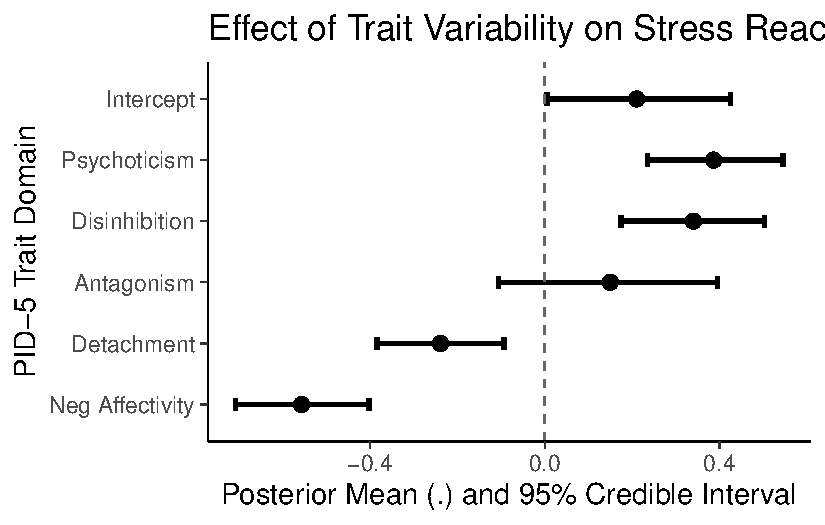
\includegraphics[keepaspectratio]{risk_files/figure-pdf/unnamed-chunk-54-1.pdf}}

\begin{Shaded}
\begin{Highlighting}[]
\NormalTok{post\_beta}\SpecialCharTok{$}\NormalTok{direction }\OtherTok{\textless{}{-}} \FunctionTok{ifelse}\NormalTok{(post\_beta}\SpecialCharTok{$}\NormalTok{lower\_95 }\SpecialCharTok{\textgreater{}} \DecValTok{0}\NormalTok{, }\StringTok{"positive"}\NormalTok{,}
                               \FunctionTok{ifelse}\NormalTok{(post\_beta}\SpecialCharTok{$}\NormalTok{upper\_95 }\SpecialCharTok{\textless{}} \DecValTok{0}\NormalTok{, }\StringTok{"negative"}\NormalTok{, }\StringTok{"uncertain"}\NormalTok{))}

\FunctionTok{ggplot}\NormalTok{(post\_beta, }\FunctionTok{aes}\NormalTok{(}\AttributeTok{x =}\NormalTok{ mean, }\AttributeTok{y =}\NormalTok{ label, }\AttributeTok{color =}\NormalTok{ direction)) }\SpecialCharTok{+}
  \FunctionTok{geom\_point}\NormalTok{(}\AttributeTok{size =} \DecValTok{3}\NormalTok{) }\SpecialCharTok{+}
  \FunctionTok{geom\_errorbarh}\NormalTok{(}\FunctionTok{aes}\NormalTok{(}\AttributeTok{xmin =}\NormalTok{ lower\_95, }\AttributeTok{xmax =}\NormalTok{ upper\_95), }\AttributeTok{height =} \FloatTok{0.2}\NormalTok{, }\AttributeTok{linewidth =} \DecValTok{1}\NormalTok{) }\SpecialCharTok{+}
  \FunctionTok{geom\_vline}\NormalTok{(}\AttributeTok{xintercept =} \DecValTok{0}\NormalTok{, }\AttributeTok{linetype =} \StringTok{"dashed"}\NormalTok{, }\AttributeTok{color =} \StringTok{"gray40"}\NormalTok{) }\SpecialCharTok{+}
  \FunctionTok{scale\_color\_manual}\NormalTok{(}\AttributeTok{values =} \FunctionTok{c}\NormalTok{(}
    \StringTok{"positive"} \OtherTok{=} \StringTok{"firebrick3"}\NormalTok{,}
    \StringTok{"negative"} \OtherTok{=} \StringTok{"steelblue"}\NormalTok{,}
    \StringTok{"uncertain"} \OtherTok{=} \StringTok{"gray40"}
\NormalTok{  )) }\SpecialCharTok{+}
  \FunctionTok{labs}\NormalTok{(}
    \AttributeTok{x =} \StringTok{"Posterior Mean (β) and 95\% Credible Interval"}\NormalTok{,}
    \AttributeTok{y =} \StringTok{"PID{-}5 Trait Domain"}\NormalTok{,}
    \AttributeTok{title =} \StringTok{"Effect of EMA Trait Variability on Stress Reactivity"}\NormalTok{,}
    \AttributeTok{color =} \StringTok{"Direction of Association"}
\NormalTok{  ) }
\end{Highlighting}
\end{Shaded}

\pandocbounded{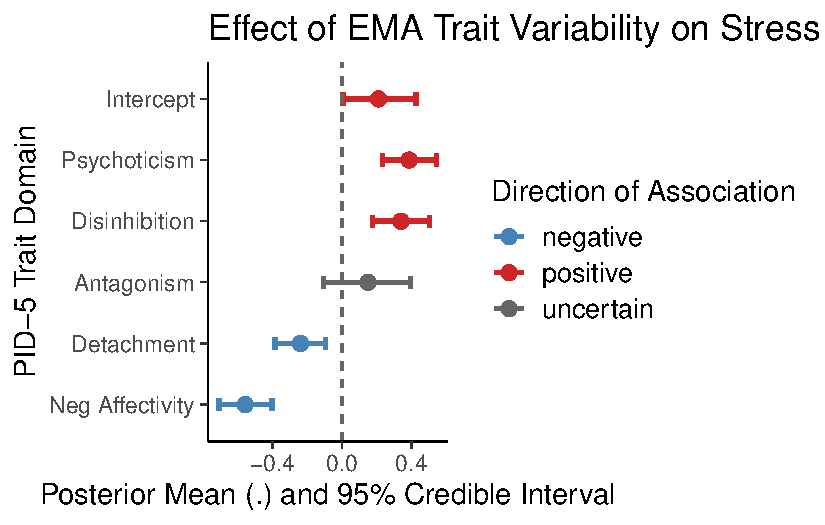
\includegraphics[keepaspectratio]{risk_files/figure-pdf/unnamed-chunk-55-1.pdf}}




\end{document}
